
\documentclass{disser}
\usepackage[T2A]{fontenc}
\usepackage[english, russian]{babel}

\makeatletter
\renewcommand\tableofcontents{%
  \@starttoc{toc}%
  \thispagestyle{plain} % Применить стиль
}
\makeatother


\usepackage{graphicx}
\graphicspath{ {./images/} }

\usepackage{blindtext}
\usepackage[figurename=Рисунок]{caption}
\usepackage{indentfirst}

% Геометрия страницы и графика
\usepackage[left=3cm, right=1cm, top=2cm, bottom=2cm]{geometry} % поля страницы
\usepackage{pdfpages} % вставка pdf-страниц

% Таблицы
\usepackage{array} % расширенные возможности для работы с таблицами
\usepackage{tabularx} % автоматический подбор ширины столбцов
\usepackage{dcolumn} % выравнивание чисел по разделителю

% Математика
\usepackage{bm} % полужирное начертание для математических символов
\usepackage{amsmath} % дополнительные математические возможности
\usepackage{amssymb} % дополнительные математические символы

% Библиография и ссылки
\usepackage{cite} % поддержка цитирования

% Прочее
\usepackage{color} % работа с цветом
\usepackage{epstopdf} % конвертация eps в pdf
\usepackage{multirow} % объединение ячеек таблиц по вертикали
\usepackage{afterpage} % вставка материала после текущей страницы
\usepackage[font={normal}]{caption} % настройка подписей к рисункам и таблицам
\usepackage[onehalfspacing]{setspace} % полуторный интервал
\usepackage{fancyhdr} % установка колонтитулов
% Основные настройки
\pagestyle{fancy}
\fancyhf{} % Очистить все колонтитулы
\renewcommand{\headrulewidth}{0pt} % Убрать линию в верхнем колонтитуле
\fancyfoot[C]{\thepage} % Номер страницы внизу по центру
\usepackage{hyperref} % создание гиперссылок
\usepackage{listings} % поддержка вставки исходного кода
% \usepackage{ragged2e}

%Define the listing package
\usepackage{color} %use color
\definecolor{mygreen}{rgb}{0,0.6,0}
\definecolor{mygray}{rgb}{0.5,0.5,0.5}
\definecolor{mymauve}{rgb}{0.58,0,0.82}
 
%Customize a bit the look
\lstset{ %
backgroundcolor=\color{white}, % choose the background color; you must add \usepackage{color} or \usepackage{xcolor}
basicstyle=\footnotesize, % the size of the fonts that are used for the code
breakatwhitespace=false, % sets if automatic breaks should only happen at whitespace
breaklines=true, % sets automatic line breaking
captionpos=b, % sets the caption-position to bottom
commentstyle=\color{mygreen}, % comment style
deletekeywords={...}, % if you want to delete keywords from the given language
escapeinside={\%*}{*)}, % if you want to add LaTeX within your code
extendedchars=true, % lets you use non-ASCII characters; for 8-bits encodings only, does not work with UTF-8
frame=single, % adds a frame around the code
keepspaces=true, % keeps spaces in text, useful for keeping indentation of code (possibly needs columns=flexible)
keywordstyle=\color{blue}, % keyword style
% language=Octave, % the language of the code
morekeywords={*,...}, % if you want to add more keywords to the set
numbers=left, % where to put the line-numbers; possible values are (none, left, right)
numbersep=5pt, % how far the line-numbers are from the code
numberstyle=\tiny\color{mygray}, % the style that is used for the line-numbers
rulecolor=\color{black}, % if not set, the frame-color may be changed on line-breaks within not-black text (e.g. comments (green here))
showspaces=false, % show spaces everywhere adding particular underscores; it overrides 'showstringspaces'
showstringspaces=false, % underline spaces within strings only
showtabs=false, % show tabs within strings adding particular underscores
stepnumber=1, % the step between two line-numbers. If it's 1, each line will be numbered
stringstyle=\color{mymauve}, % string literal style
tabsize=2, % sets default tabsize to 2 spaces
title=\lstname % show the filename of files included with \lstinputlisting; also try caption instead of title
}
%END of listing package%
 
\definecolor{darkgray}{rgb}{.4,.4,.4}
\definecolor{purple}{rgb}{0.65, 0.12, 0.82}
 
%define Javascript language
\lstdefinelanguage{JavaScript}{
keywords={typeof, new, true, false, catch, function, return, null, catch, switch, var, if, in, while, do, else, case, break},
keywordstyle=\color{blue}\bfseries,
ndkeywords={class, export, boolean, throw, implements, import, this},
ndkeywordstyle=\color{darkgray}\bfseries,
identifierstyle=\color{black},
sensitive=false,
comment=[l]{//},
morecomment=[s]{/*}{*/},
commentstyle=\color{purple}\ttfamily,
stringstyle=\color{red}\ttfamily,
morestring=[b]',
morestring=[b]"
}
 
\lstset{
language=JavaScript,
extendedchars=true,
basicstyle=\footnotesize\ttfamily,
showstringspaces=false,
showspaces=false,
numbers=left,
numberstyle=\footnotesize,
numbersep=9pt,
tabsize=2,
breaklines=true,
showtabs=false,
captionpos=b
}
 


% Создание нового типа столбца для выравнивания содержимого по центру
\newcommand{\PreserveBackslash}[1]{\let\temp=\\#1\let\\=\temp}
\newcolumntype{C}[1]{>{\PreserveBackslash\centering}p{#1}}

% Настройка подписей к изображениям и таблицам
\captionsetup{format=hang,labelsep=period}

% Использование полужирного начертания для векторов
\let\vec=\mathbf

% Установка глубины оглавления
\setcounter{tocdepth}{2}

\newcommand{\mychapter}[1]{%
  \refstepcounter{chapter}%
  \chapter*{\thechapter\quad#1}%
  \addcontentsline{toc}{chapter}{{\normalfont\thechapter\quad\MakeUppercase{#1}}}%
}

\newcommand{\mychapternonum}[1]{%
  \chapter*{\MakeUppercase{#1}}%
  \addcontentsline{toc}{chapter}{\normalfont\MakeUppercase{#1}}%
}


\newcommand{\mysection}[1]{%
  \refstepcounter{section}%
  \section*{\centering\bfseries\thesection\quad #1}
  \addcontentsline{toc}{section}{\protect\numberline{\thesection}#1}%  % Обычный в оглавлении
}

\newcommand{\mysubsection}[1]{%
  \refstepcounter{subsection}%
  \subsection*{\bfseries\thesubsection\quad #1}%  % Жирный текст в подсекции
  \addcontentsline{toc}{subsection}{\protect\numberline{\thesubsection}#1}%  % Обычный текст в оглавлении
}

\newcommand{\mysubsubsection}[1]{%
  \refstepcounter{subsubsection}%
  \subsubsection*{{\normalfont\thesubsubsection\quad#1}}%
  \addcontentsline{toc}{subsubsection}{{\normalfont\thesubsubsection\quad#1}}%
}



\renewcommand{\thetable}{\arabic{table}}

\DeclareCaptionLabelFormat{dash}{#1~#2~--- } % определяем формат: имя, номер и тире
\captionsetup[table]{%
  labelformat=dash, 
  labelsep=none, 
  justification=raggedright,  % выравнивание по левому краю
  singlelinecheck=false       % для одиночных строк тоже левое выравнивание
}

\newcommand{\myparagraph}[1]{\paragraph{#1}\mbox{}\\}




\renewcommand{\thefigure}{\arabic{figure}}

\usepackage[font=normal]{caption}
\DeclareCaptionLabelFormat{figdash}{Рисунок~#2~– }
\captionsetup[figure]{labelformat=figdash, labelsep=none, justification=raggedright}

\begin{document}


\includepdf[pages={1-5}]{Title.pdf}
\newpage
\begin{center}
  \textbf{\large АННОТАЦИЯ}
\end{center}
Текст аннотации

\newpage
\begin{center}
  \textbf{\large СОДЕРЖАНИЕ}
\end{center}
\tableofcontents
\thispagestyle{plain} % Гарантирует стиль для текущей страницы
\newpage

\mysection{Предметная область и проблема}

\mysubsection{Описание предметной области}
В настоящее время в сфере образования, в частности, в сегменте частных школ и индивидуального обучения, растет запрос к современному подходу в организации учебного процесса. Преподаватели тратят значительное время на рутинные задачи: формирование расписаний, учет посещаемости, контроль оплаты занятий и коммуникацию с учениками. При этом существующие инструменты часто оказываются либо слишком сложными (например, системы управления обучением — LMS), либо недостаточно специализированными под нужды групповых занятий.

Разработка веб-приложения для администрирования групповых занятий направлена на решение этих проблем. Цель проекта — создать интуитивно понятную платформу, которая объединит функции планирования, учета, финансового контроля и коммуникации, адаптированную под потребности преподавателей и частных образовательных учреждений. Приложение позволит автоматизировать ключевые процессы, снизив нагрузку на пользователей и повысив прозрачность учебного процесса для учеников и их родителей.

Для достижения поставленной цели были выделены следующие задачи:

\begin{enumerate}
    \item Проанализировать предметную область.
    \item Провести анализ целевой аудитории.
    \item Провести анализ конкурентов и аналолги.
    \item Определиться с функциональными и нефункциональными требованиями.
    \item Спроектировать и описать бизнес процессы.
    \item Спроектировать и разработать систему.
    \item Спроектировать пользовательский интерфейс.
    \item Протестировать разработанную систему на реальных потребителях.
    \item Сделать выводы о результатах применения системы и выполненных целях.
\end{enumerate}

\mysubsection{Целевая аудитория}
Целевая аудитория — это группа потенциальных потребителей какого-то продукта, люди, которые вероятнее всего заинтересуются товаром или услугой.

Для определения портрета целевой аудитории был проведен опрос, направленный на представителей образовательной сферы деятельности. Респондентам было представлено 9 вопросов, по результатам которым можно оценить портрет целевой аудитории, проблемы с которыми ониа сталкивается, а также понять основной запрос целевой аудитории в рамках образовательного процесса.

В опросе приняли участие 37 респондентов, подавляющее число из которых - представители молодного поколения, в возрасте от 20 до 30 лет. 

{
    \centering
    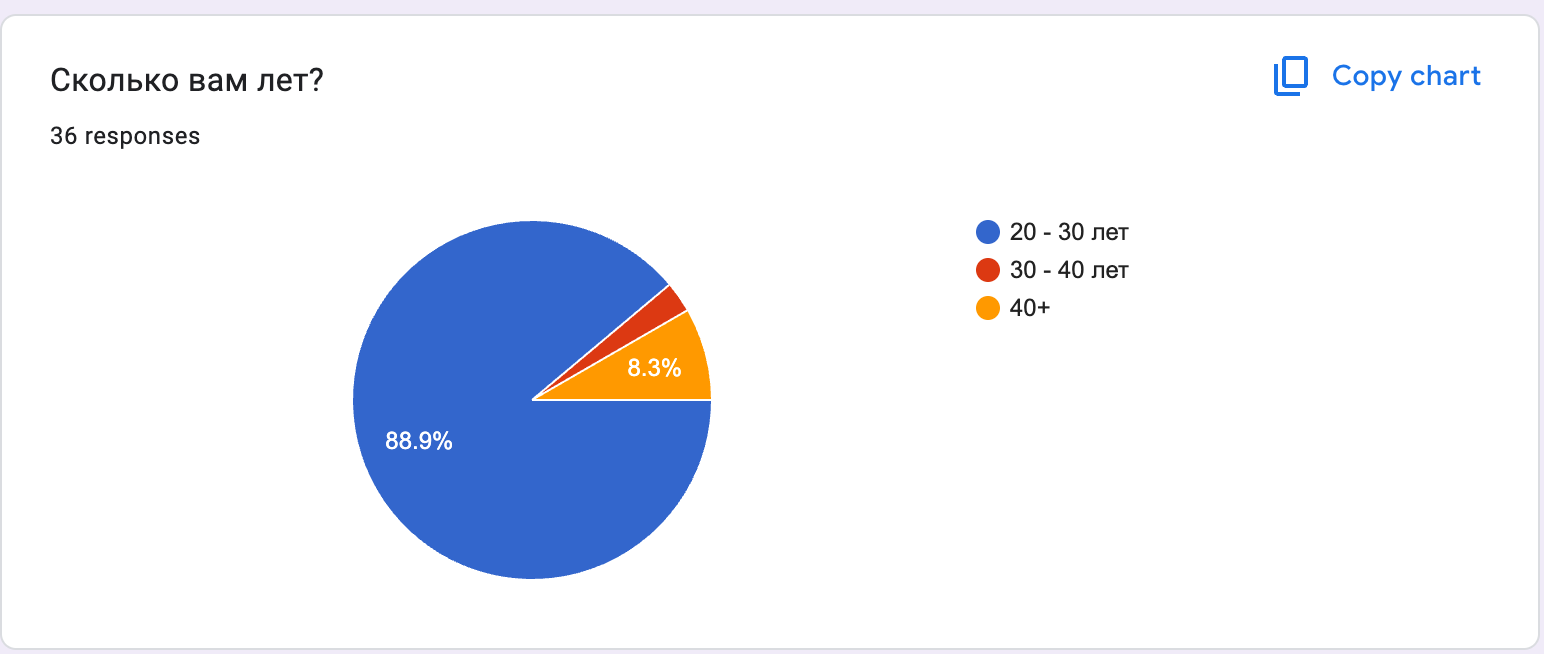
\includegraphics[width=0.8\linewidth]{images/pool/question_1.png}
    \captionof{figure}{Результаты демографии.}
    \label{fig:enter-label}
}

Касаемо профессии, больше половины принявших участие респондентов являются частными репетиторами. На 2 месте по частоте - преподаватели частных школ.

{
    \centering
    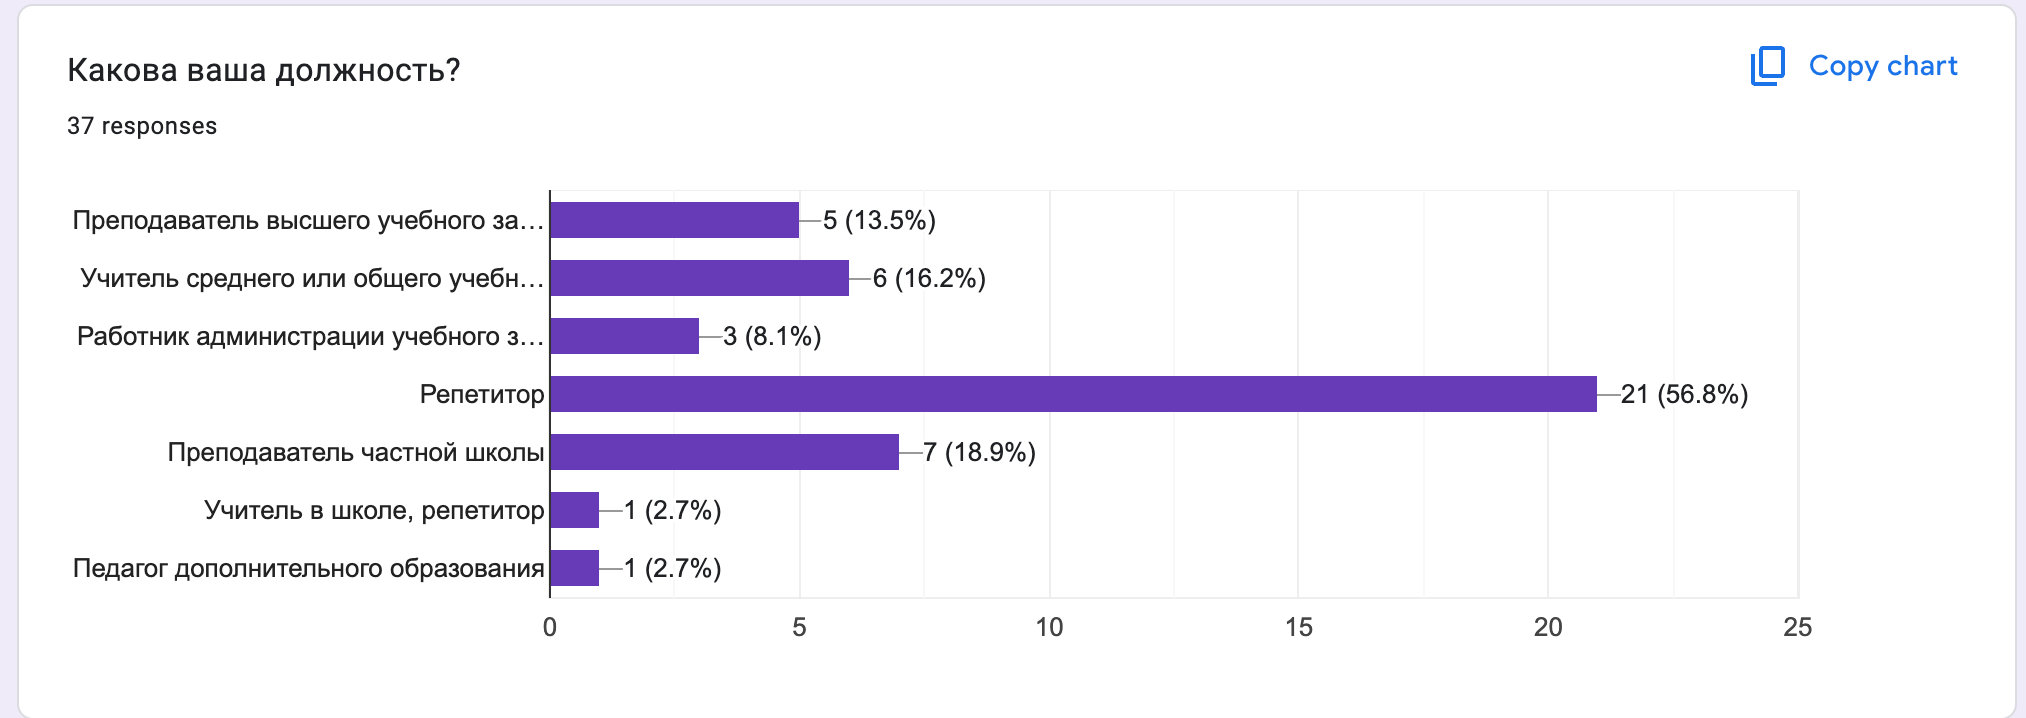
\includegraphics[width=0.8\linewidth]{images/pool/question_2.png}
    \captionof{figure}{Статистика по профессии.}
    \label{fig:enter-label}
}

Благодаря этой метрике, можно сегментировать ответы и определить в какой сфере самые популярные трудности. 

Далее, следующий вопрос направлен на выявление опытности респондента в сфере образования.  В результате 45.9\% опрошенных имеют опыт от 2 до 5 лет, 40.5\% только начинают свой путь в образовательной деятельности, и лишь 13\% опрошенных имеют более серьезный опыт.
{
    \centering
    \fbox{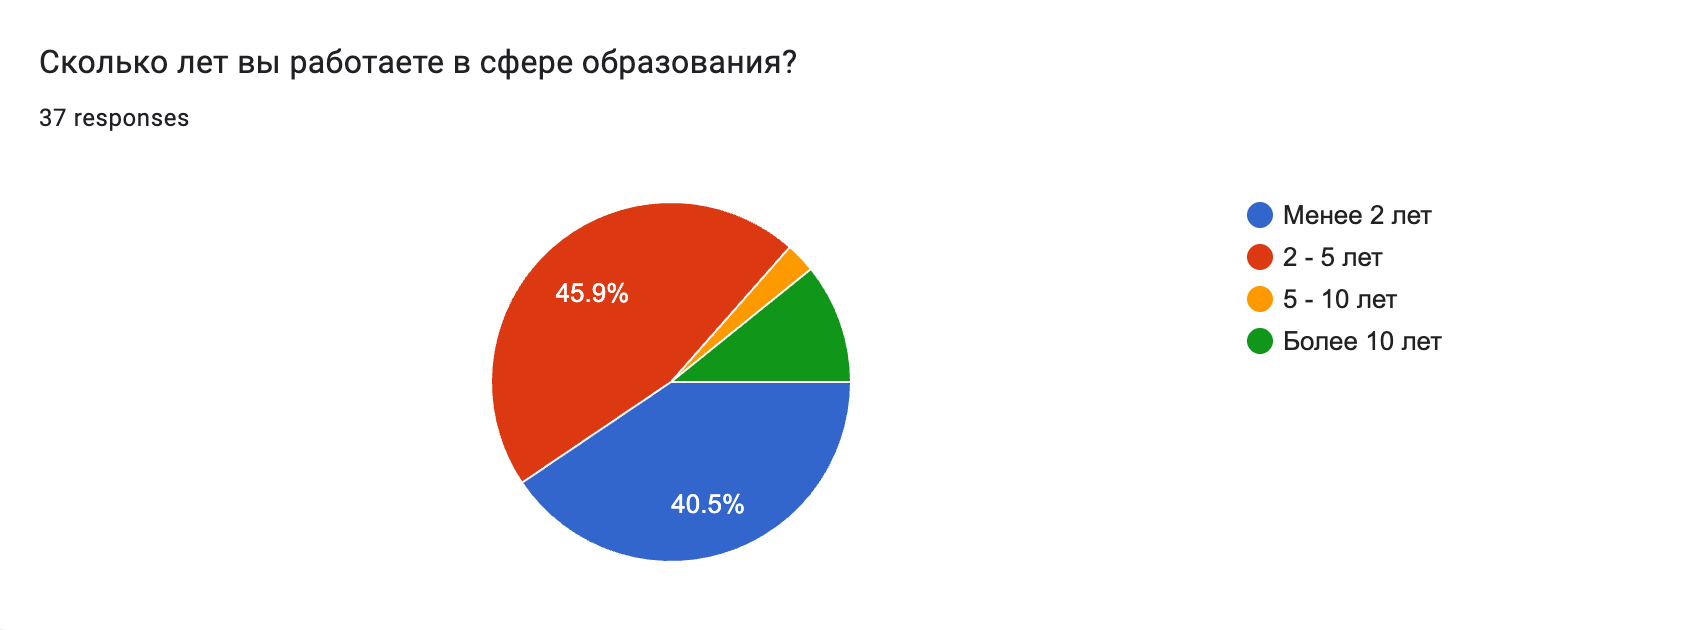
\includegraphics[width=0.8\linewidth]{images/pool/question_3.png}}
    \captionof{figure}{Опыт респондентов.}
    \label{fig:enter-label}
}

Следующий вопрос был направлен на выяснение самых времязатратных задач в работе респондентов.

Из рисунка 4 можно сделать вывод о том, что самой времязатратной задачей являетсяя загрузка учебных материалов, составление и корректировка расписания и коммуникация с учениками. Также из общей таблицы ответом можно получить ифномацию о том, что с проблемой загрузки учебных материалов сталкиваются в основном репетиторы, когда с проблемой коммуникации сталкиваются в основном учителя среднего образования, а учет посещаемости является главной проблемой преподавателей частных школ. Это говорит о том, что эти процессы требуют автоматизации.

{
    \centering
    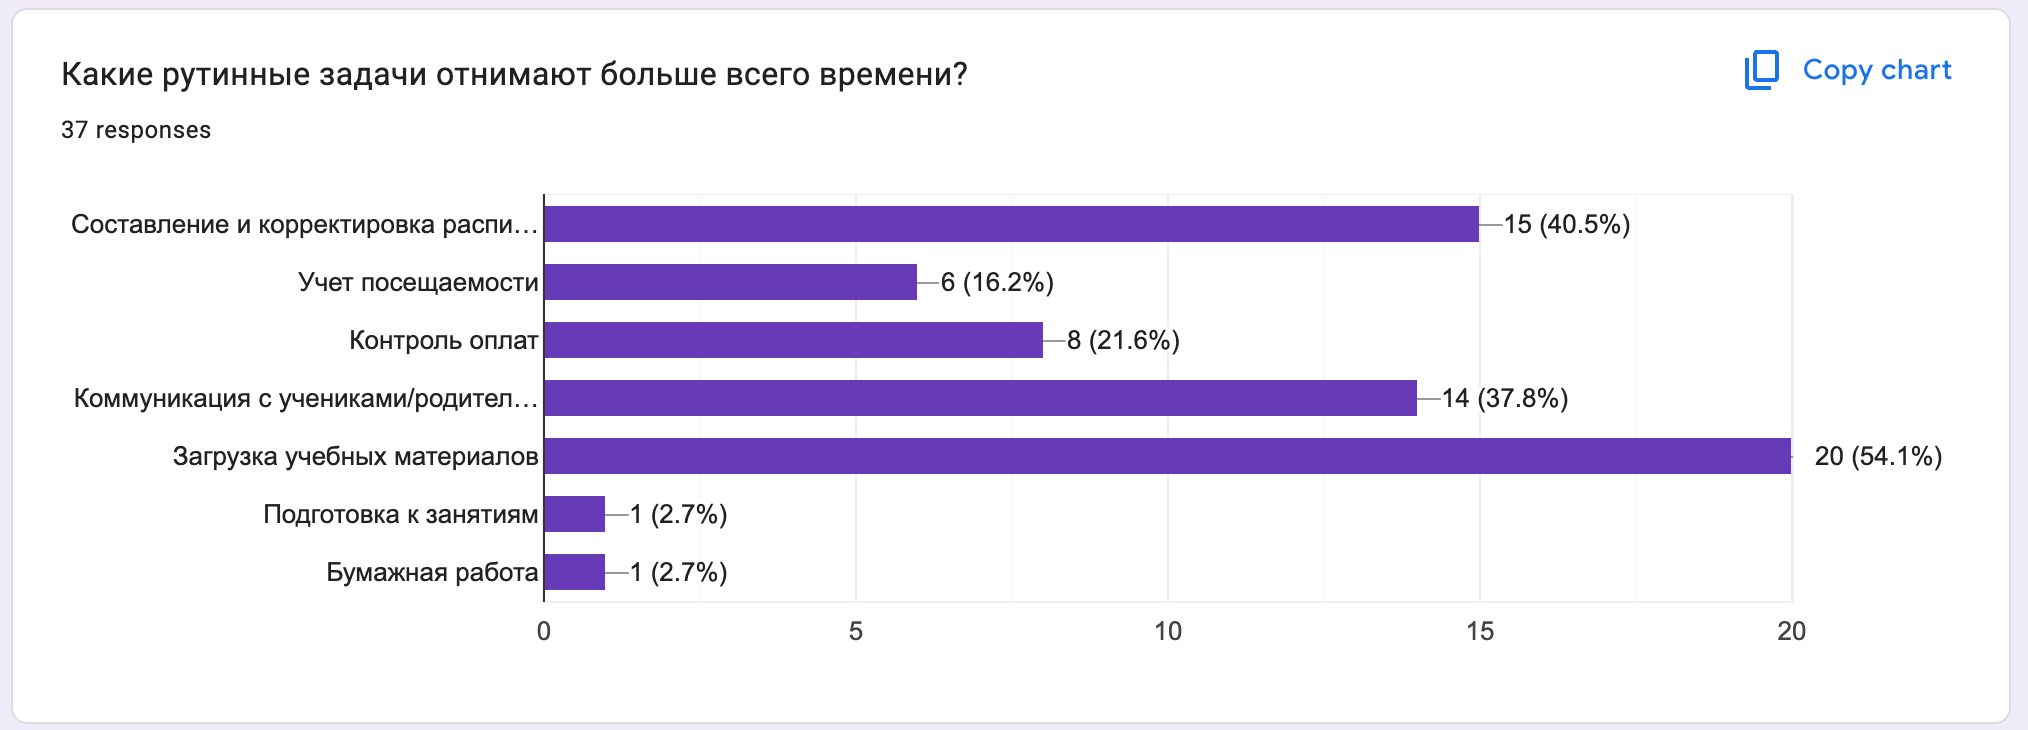
\includegraphics[width=0.8\linewidth]{images/pool/question_4.png}
    \captionof{figure}{Самые времязатратные задачи.}
    \label{fig:enter-label}
}

На рисунке 5 представлены результаты вопроса, направленного на выявление инструментария, которым пользуются респонденты сейчас для решения своих повседневных задач. 

{
    \centering
    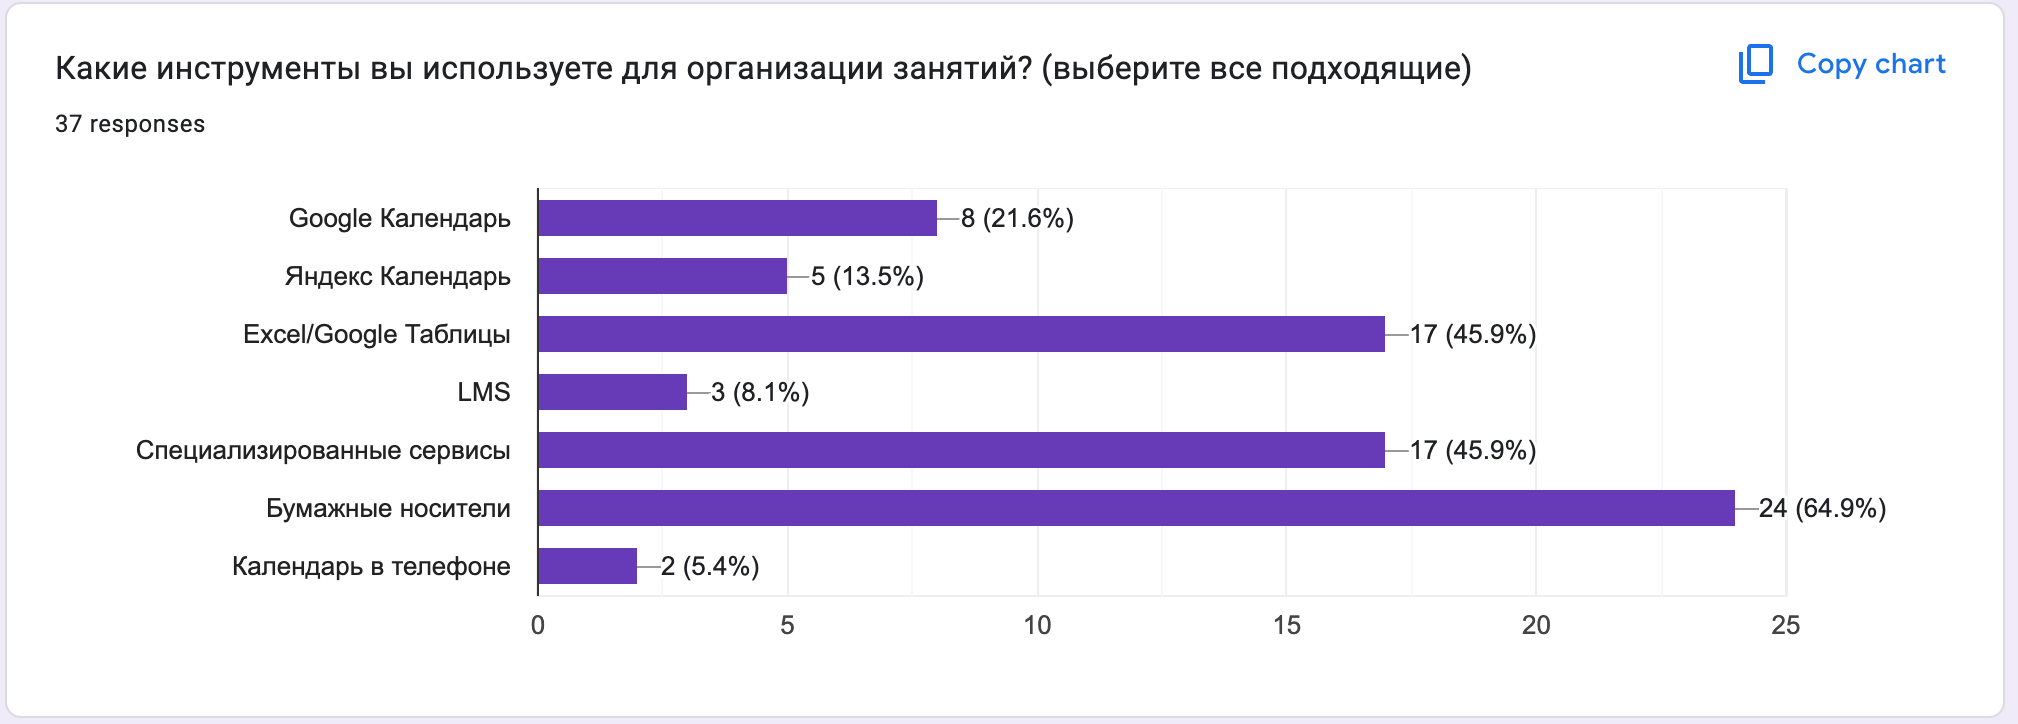
\includegraphics[width=0.8\linewidth]{images/pool/question_5.png}
    \captionof{figure}{Наиболее используемые инструменты}
    \label{fig:enter-label}
}

Из ответов вижно, что 64\% опрошенных предпочитают вести учет своей деятельности на бумаге и лишь 35\% предпочитают использовать электронные носители. Это дает сигнал о том, что многие респонденты не готовы использовать специализированные сервисы, поскольку, как показано на рисунке 7, эти же респонденты, что выбрали основной инструмент - бумагу, ответили, что главной их проблемой является дублирование и потеря информации. Исходя из этого можно сделать вывод о том, что эта часть целевой аудитории желает перейти от традиционног ведения учета на бумаге к более подходящему решению и испытывает трудности.

Также, из рисунка 5 можно сделать простой вывод о том, что хоть 45\% ответили, что используют специлизированные сервисы, также используют Excel. Это говорит о фрагментации данных. Респонденты вынуждены использовать множество сервисов одновременно и это подтверждает нишу моего решения.

На рисунке 6 представлен вопрос о владения компьютером. 

{
    \centering
    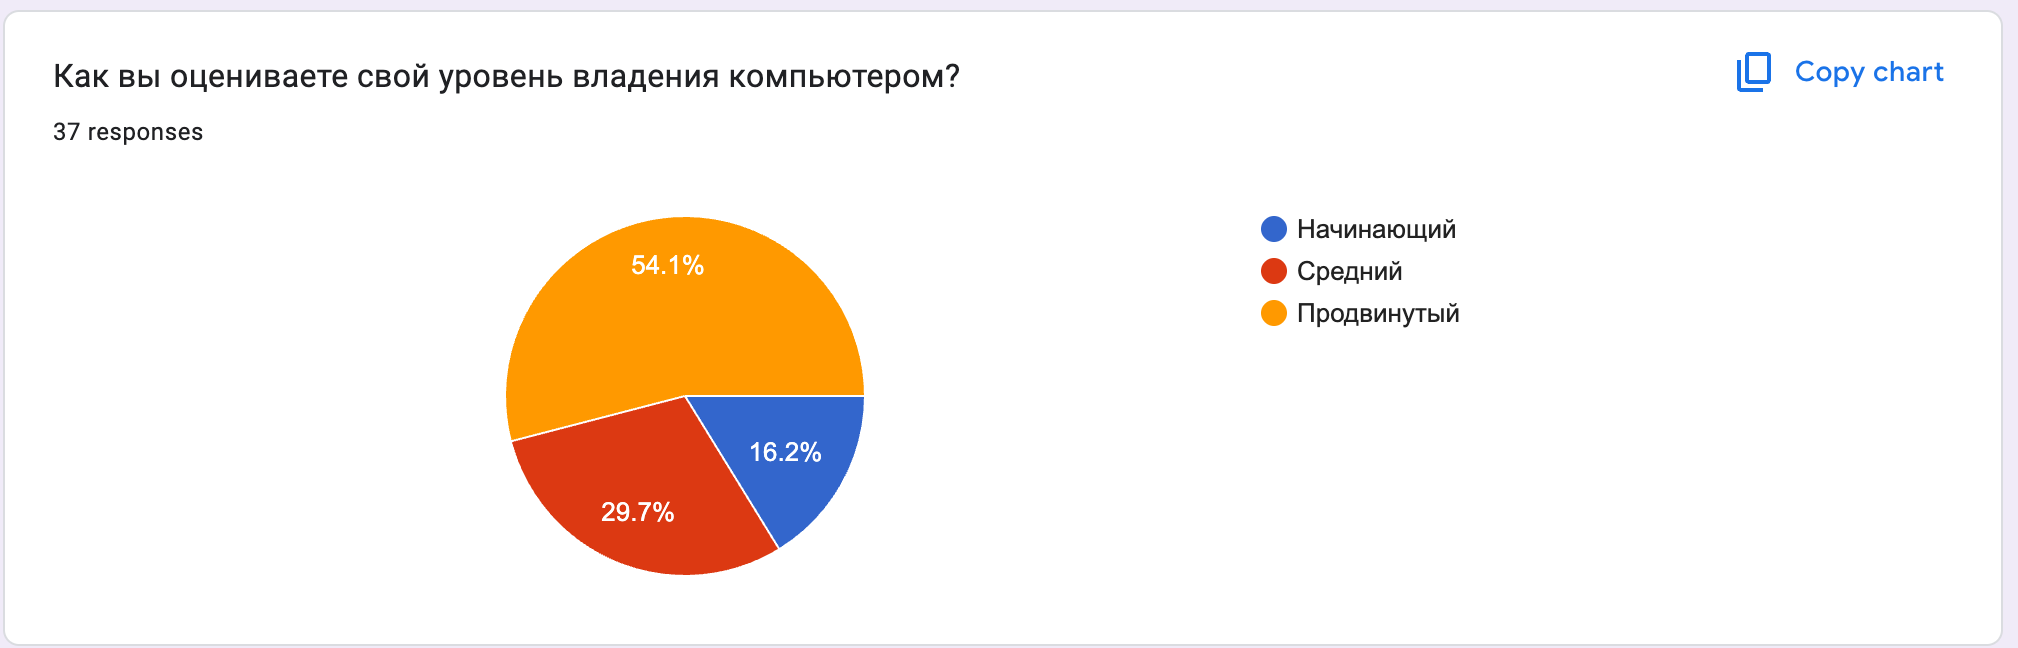
\includegraphics[width=0.8\linewidth]{images/pool/question_6.png}
    \captionof{figure}{Уровень владения компьютером.}
    \label{fig:enter-label}
}
Из результатов вопроса можно уверенно сказать, что основная часть целевой аудитории имеют высокий или средний уровень владения компьютером. Это значит, что интерфейс системы должен быть интутивно понятным и не вызывать большой когнитивной нагрузки.

Вопрос 7 нацелен на выявление удовлетворенности целевой аудитории с сервисами, которые они используют сейчас.

{
    \centering
    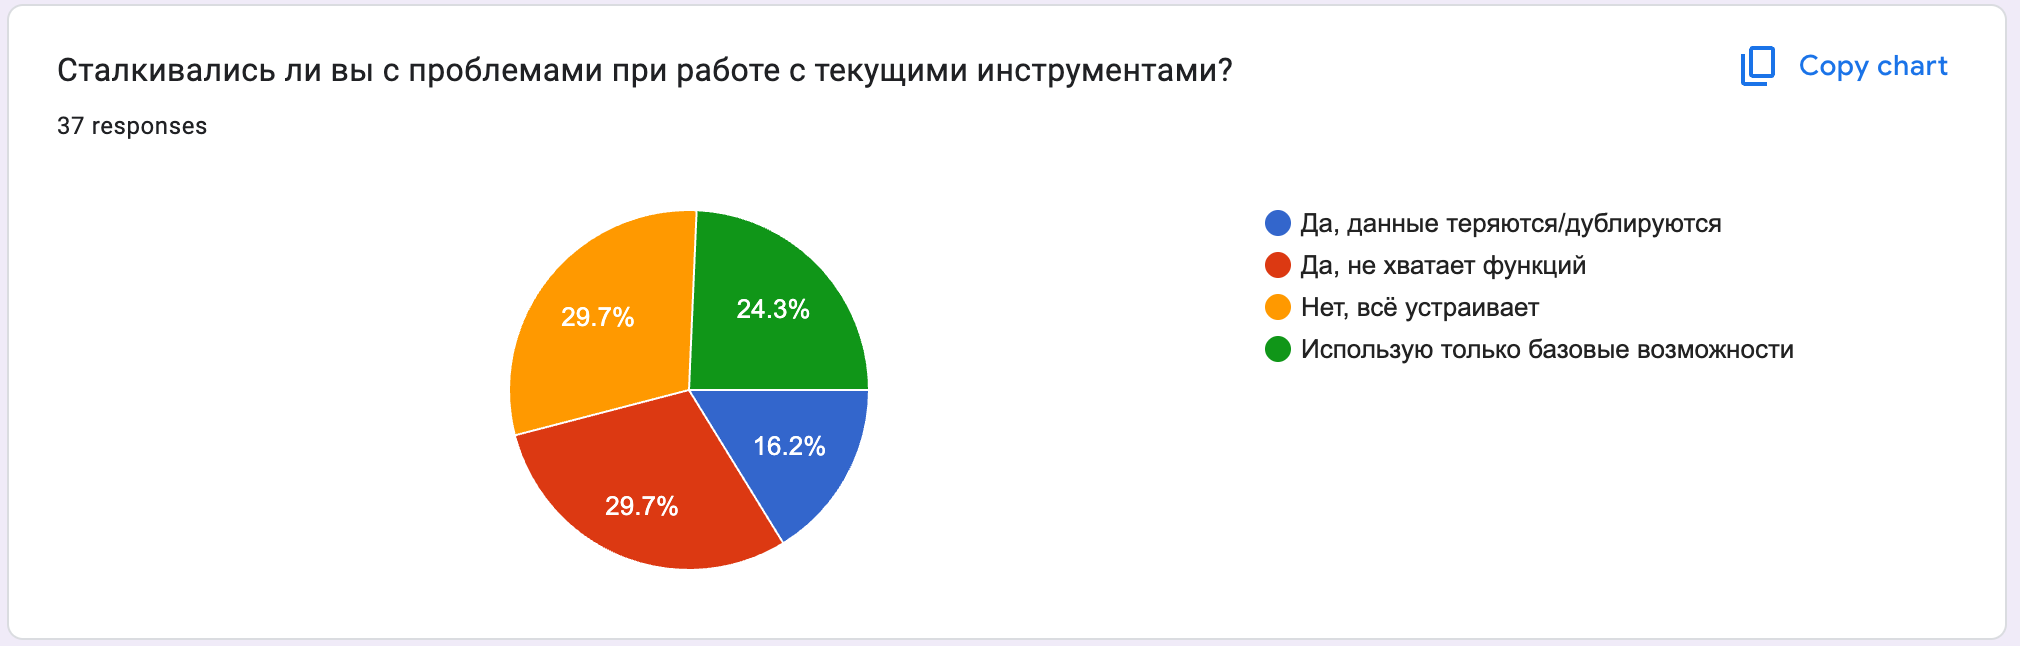
\includegraphics[width=0.8\linewidth]{images/pool/qustion_7.png}
    \captionof{figure}{Удовлетворенность текущими решениями.}
    \label{fig:enter-label}
}

Здесь видно, что мнения респондентов разделились. Около трети респондентов ответили, что им не хватает некоторого функционала, 16\% заявлили им не хватает критически важного функционала и испытывают проблемы с хранением информации. Это дает основание полагать, что мое решение будет особенно актуально для минимизирования ручного труда.

По итогам 8 вопроса, представленного на рисунке 8, можно сделать вывод о том, что весь перечисленный функционал востребован среди целевой аудитории. Из сводной таблицы, можно сделать вывод о том, что те респонденты, которые указали своей главной проблемой "Составление и корректировка расписания", использующие Excel больше всего выбрали желаемый функционал "Автоматическое расписание с повторяемыми занятиями", а также "Ведение финансовой отчетности". 
Также, те респонденты, уровень владения компьютером которых явлется низким или средним, ответили, что хотели бы видеть адаптированную версию сервиса под мобильные устройства.
А гибкие настройки доступа, разделение групп обучающихся на открытые и закрытые, отметили в основном репетиторы и преподаватели частных школ и заведений.

{
    \centering
    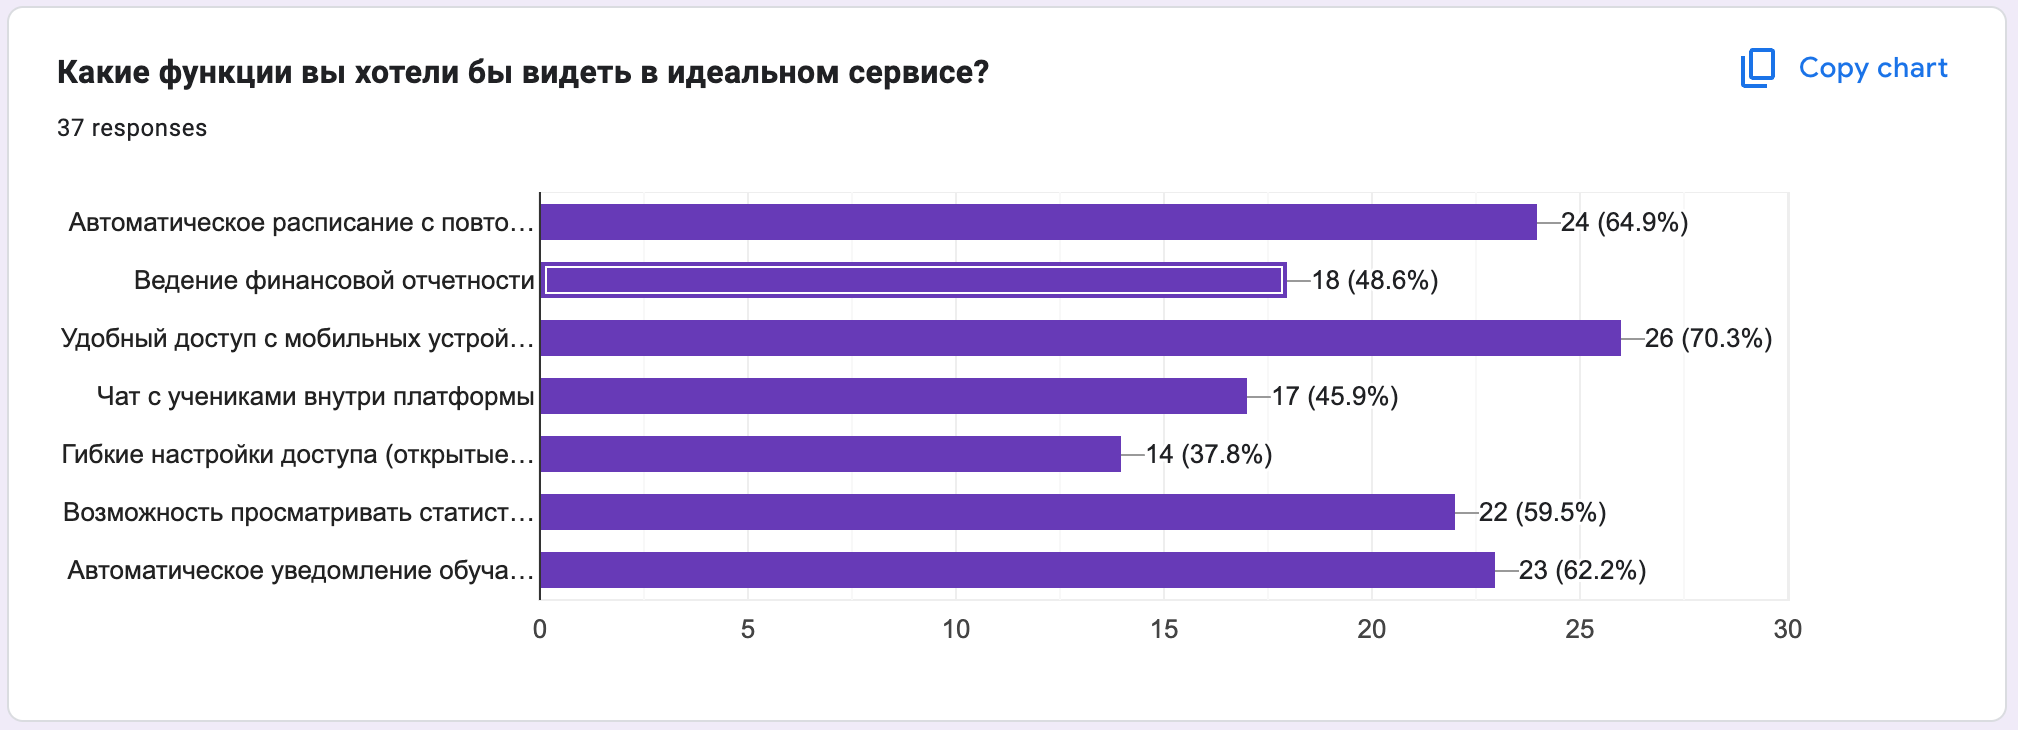
\includegraphics[width=0.8\linewidth]{images/pool/question_8.png}
    \captionof{figure}{Функции идеального сервиса}
    \label{fig:enter-label}
}


Из результатов проведенного опроса, можно составить портрет среднестистического пользователя системы администирования групповых занятий. 
 
Портрет ЦА:
\begin{itemize}
    \item возраст: 25–35 лет;
    \item опыт работы: 2-10 лет;
    \item техническая подготовка: средний уровень.
Многие не имеют опыта работы с профессиональными CRM или LMS, но активно используют базовые инструменты (Яндекс Календарь, Excel, мессенджеры).
\end{itemize}

Потребности:

\begin{itemize}
    \item быстрое создание групп и расписаний без ручного ввода данных;
    \item учет посещаемости с возможностью отметки в реальном времени;
    \item автоматический расчет доходов;
    \item доступ к статистике (посещаемость, оплаты, успеваемость);
\end{itemize}

Проблемы, с которыми сталкиваются:

\begin{itemize}
    \item фрагментация инструментов: расписание в одном месте, оплаты — в другом, общение — в мессенджере;
    \item сложности с контролем задолженностей учеников;
    \item отсутствие единого пространства для работы с группами;
    \item недостаток коммуникации с обучающимися.
\end{itemize}

Также, для автоматизации процесса ведения груп, а также расширения функциональности системы, проанализирована вторичная аудитория: обучающиеся.

Портрет ЦА:

\begin{itemize}
    \item возраст обучающихся: 12–25 лет
    \item техническая подготовка: средняя. Хорошо владеют компьютером и телефоном, но не имеют навыков работы в профессиональных CRM системах и LMS
\end{itemize}

Потребности:

\begin{itemize}
    \item просмотр расписания занятий и домашних заданий;
    \item запись на групповые или индивидуальные занятия;
    \item доступ к истории оплат и посещаемости.
\end{itemize}

Проблемы, с которыми сталкиваются:

\begin{itemize}
    \item необходимость уточнять расписание у преподавателя;
    \item отсутствие прозрачности в оплатах.
\end{itemize}

\mysubsection{Анализ требований целевой аудитории}

По сформерованным портретам основной целевой аудитории можно определиться с списоком функциональных и нефункциональных требований к системе, которые будут нацелены на улучшение пользовательского опыта и решение главных задач целевой аудитории.


\mysubsection{Анализ аналогов и конкурентов}

К сожалению, сегодня, большинство преподавателей и репетиторов предпочитают использовать excel таблицы.
Преимущества:
\begin{itemize}
    \item Приемственность. 
    
    Многие используют Excel поскольку десятилетиями использовали его для выполнения всех своих рутинных задач и попросту не хотят переходить на что-то более новое.
    \item Доступность. 
    
    Excel предустановлен на всех Windows устройствах и доступен сразу "из коробки". Пользователю сразу доступен весь функционал.
    \item Удобство хранения. 
    
    Некоторые xslx редакторы поддерживают облачное хранение, обеспечивая своим пользователем общим доступом с разных устройств, лишая их необходимости носить устройства накопления информации.
\end{itemize}
Недостатки:
\begin{itemize}
    \item Сбор информации. 
    
    Пользователю необхожимо вручную вводить информацию по каждому своему ученику на каждое занятие. На это тратится много времени, а также много теряется на построение коммуникации вне системы.
    \item Отсутствие целевой направленности. 
    
    Изначально excel не строился как платформа для моей целевой аудитории, а следственно не может учитывать их потребности. 
    \item Переполненость функционалом. 
    
    Excel редактор представляет собой многофункциональное приложение, способности которого только затрудняют навигацию по приложению, отвлекая тем функционалом, который не требуется для достижения целей ЦА.
\end{itemize}

Из опроса, был выявлен неочевидный, но распространенный инструмент: бумажные носитель.

Преимущества:
\begin{itemize}
    \item доступность;
    
Блокнот илил ежедневник, как правило, всегда под рукой у преподавателя.
    \item простота использования;
    
Поскольку писать могут абсолютно все, вести учет и заметки можно в любом виде.
\end{itemize}
Недостатки:
\begin{itemize}
    \item ненадежность;
    
Бумага - материал легко воспламенимый и подвержен влаге. Его крайне легко испортить, а значит быстро утратить важную ифнормацию
    \item времязатратность.
    
Ведение ежедневника обязывает тратить значительное время на орагнизацию и структуризацию данных. Это является главным недостатком, поскольку это время сегодня - главный ресурс.

\end{itemize}

Ярепетитор - прямой конкурент моей платформе, который предоставляет общий функционал создания занятий, просмотра расписания, учета заработка и оплаченных часов.
Однако, эта платформа обладает главным недостатком - односторонность использования. 
Система предоставляет функционал только для преподавателя.

Преимущества:
\begin{enumerate}
    \item Наличие календаря и вохможность вести расписание.
    \item Возможность вести статистику заработка.
    \item Многоплатформенность.
    
Сервис доступен как в веб версии, так и android и IOS приложение;
    \item наличие файлаобменника.
    
Сервис предоставляет возможность хранения заданий и материалов к занятиям.
    \item интеграция с сторонними сервисами. 
    
Сервис поддержвает авторизацию черех Google и Apple аккаунты.
\end{enumerate}

Недаостатки:
\begin{enumerate}
    \item Пользователю приходится вручную заносить каждого своего ученика в систему, а также всю информацию о нем.
    \item Пользователю приходится самому уведомлять своих учениках о переносе занятия
    \item Ученики пользователя не имеют возможности получить общую информацию о курсах и занятиях преподавателя без предварительной коммуникации. 
    
Это пораждает лишнее потраченное время на согласование времени, цены и условия проведения занятий. 
    \item Сложный и неинтуитивный интерфейс, затрудняющий использования расписания и создание занятий (рисунок 10).
\end{enumerate}

{
    \centering
    
\includegraphics[width=0.5\linewidth]{analog1.jpg}
    \captionof{figure}{Пример интерфейса аналога}
    \label{fig:enter-label}
}

Исходя из анализа конкурентов, можно выделить следующие преимущества разрабатываемого решения:

\begin{enumerate}
    \item Специализация на групповых занятиях:

Инструменты заточены под нужды преподавателей: быстрое создание групп, массовая отметка посещаемости.

    \item Все в одном месте:

Объединение расписания, оплат, коммуникации и контента избавляет от необходимости переключаться между сервисами.

    \item  Простота для не технических пользователей:

Минимум настроек, интуитивные формы, подсказки при первом входе.

    \item Финансовая прозрачность:

Автоматические напоминания об оплате, статистика доходов/расходов.

\end{enumerate}



\mysubsection{Функциональные и не функциональные требования}

Перед тем как приступить к проектированию системы, необходимо выявить все функицональные и нефункциональные требования, представленные к системе на основе опроса и конкурентов. Полученные требования отражают фактический функционал и технические особенности системы. Они включают в себы сильные стороны используемых аналогов, а также стремятся исключить повторения недостатков конкурентов.

\mysubsubsection{Функциональные требования}
Общие функциональные требования представлены на UML диаграмме 
\hypertarget{pi10}{\hyperlink{pic10_text}{рисунке 10}}

{
    \centering
    \fbox{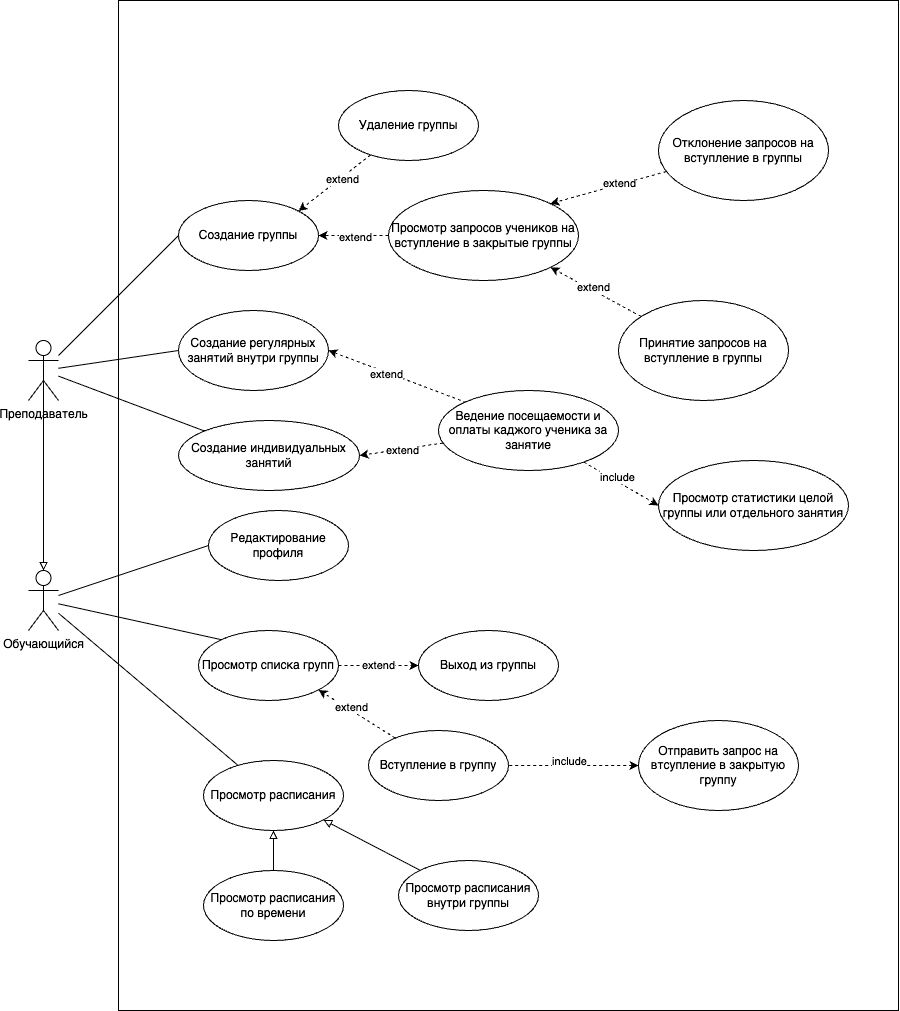
\includegraphics[scale=0.4]{images/UML.png}}
    \captionof{figure}{\hyperlink{pic10}{\hypertarget{pic10_text}{UML диаграмма по пользователям}}}
}



Для преподавателей:

\begin{enumerate}
    \item Создание групп с настройкой параметров (макс. количество учеников, стоимость занятий).
    \item Составление гибкого расписания: повторяющиеся и разовые занятия. Перенос занятий.
    \item Отметка посещаемости с возможностю добавления комменатриев.
    \item Возможность указать стоимость каждого занятия.
    \item Введение статистики по доходам.
    \item Управление контентом: добавление материалов к занятиям и домашнего задания.
    \item Уведомление учеников о переносах или отмены занятий.
\end{enumerate}

Для обучающихся:

\begin{enumerate}
    \item Личный кабинет с расписанием и историей посещений занятий.
    \item Вступление в группы преподавателей и просмотр открытых окон.
    \item Вомзожность поиска преподавателей.
\end{enumerate}

\mysubsubsection{Нефункциональные требования}

\begin{itemize}
    \item удобство интерфейса;

Современные паттерны применения дизайна, а также адаптивность под мобильные устройства
    \item безопасность;

Надежное хранение персональных данных.
    \item производительность;

Возможность посещения платформы более 1000 человек одновременно.
    \item подержкка внешних сервисов, таких как вход через Google или Yandex аккаунты.
\end{itemize}


\mysubsection{Проектирование}
\mysubsubsection{Вход в систему}
Для проектирования бизнес процессов выбрана методология описания IDEF0. Она отлично подходит для описания линейных бизнес процессов, требующие ввсеобъемлещего описания компонентов, элементов управления, действий, а также входных и выходных параметров.

Бизнес процесс входа систему представлен на рисунке 11.

{
    \centering
    
\includegraphics[width=0.5\linewidth]{images/idef0/image.png}
    \captionof{figure}{Общий бизнес процесс входа в систему в нотации IDEF0.}
    \label{fig:enter-label}
}

Этот процесс декомпозируется на регистрацию и авторизацию на уровень декомпозиции 1 и представлен на рисунке 12.

{
    \centering
    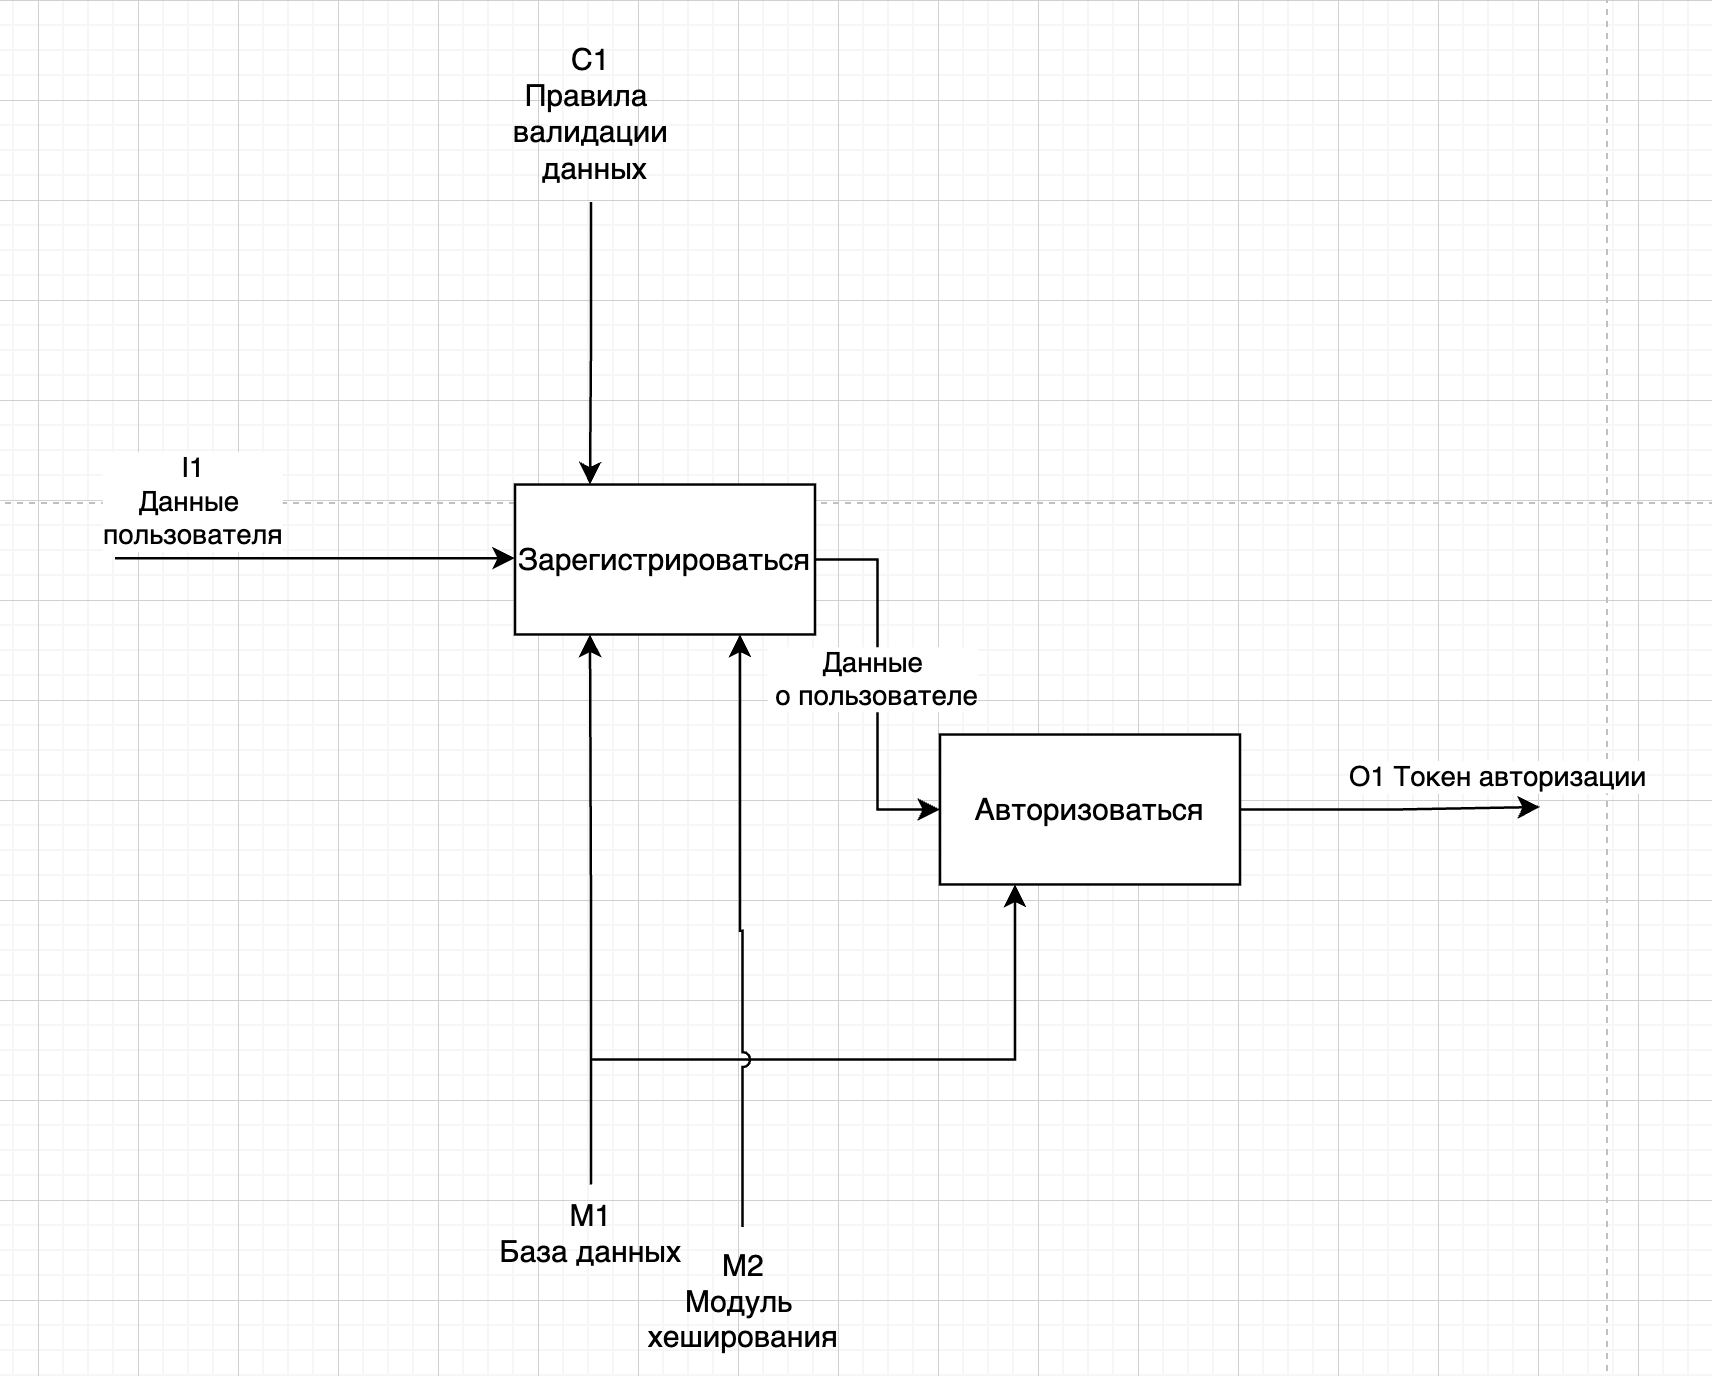
\includegraphics[width=0.5\linewidth]{images/idef0/image2.png}
    \captionof{figure}{Процесс входа в систему в нотации IDEF0 на 1 уровне декомпозиции.}
    \label{fig:enter-label}
}

Далее, рассмотрим процесс регистрации. Здесь, на вход поступают данные пользователя, а на выход id нового пользователя. Из механизмов здесь принимает участие модуль хеширования паролей, а также база данных в которой хранятся данные. Из правил, здесь присутствует Правила валидации полей

{
    \centering
    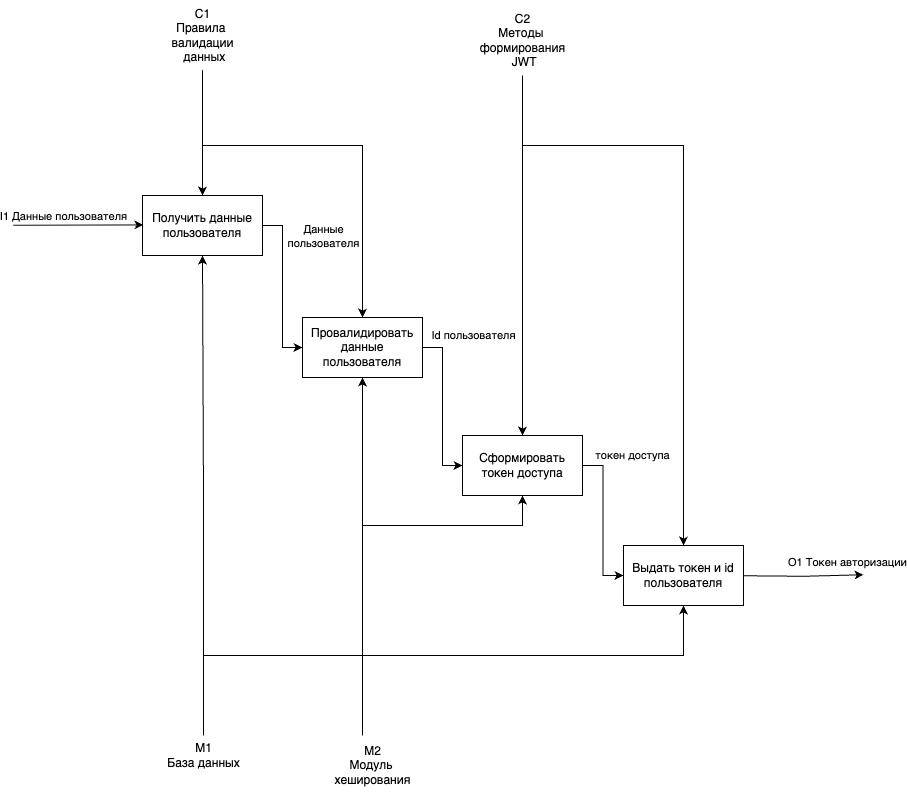
\includegraphics[width=0.7\linewidth]{images/idef0/image3.png}
    \captionof{figure}{Процесс регистрации пользователя в нотации IDEF0.}
    \label{fig:enter-label}
}

В процессе регистарции существует процесс валидации, декомпозированный на рисунке 14.

{
    \centering
    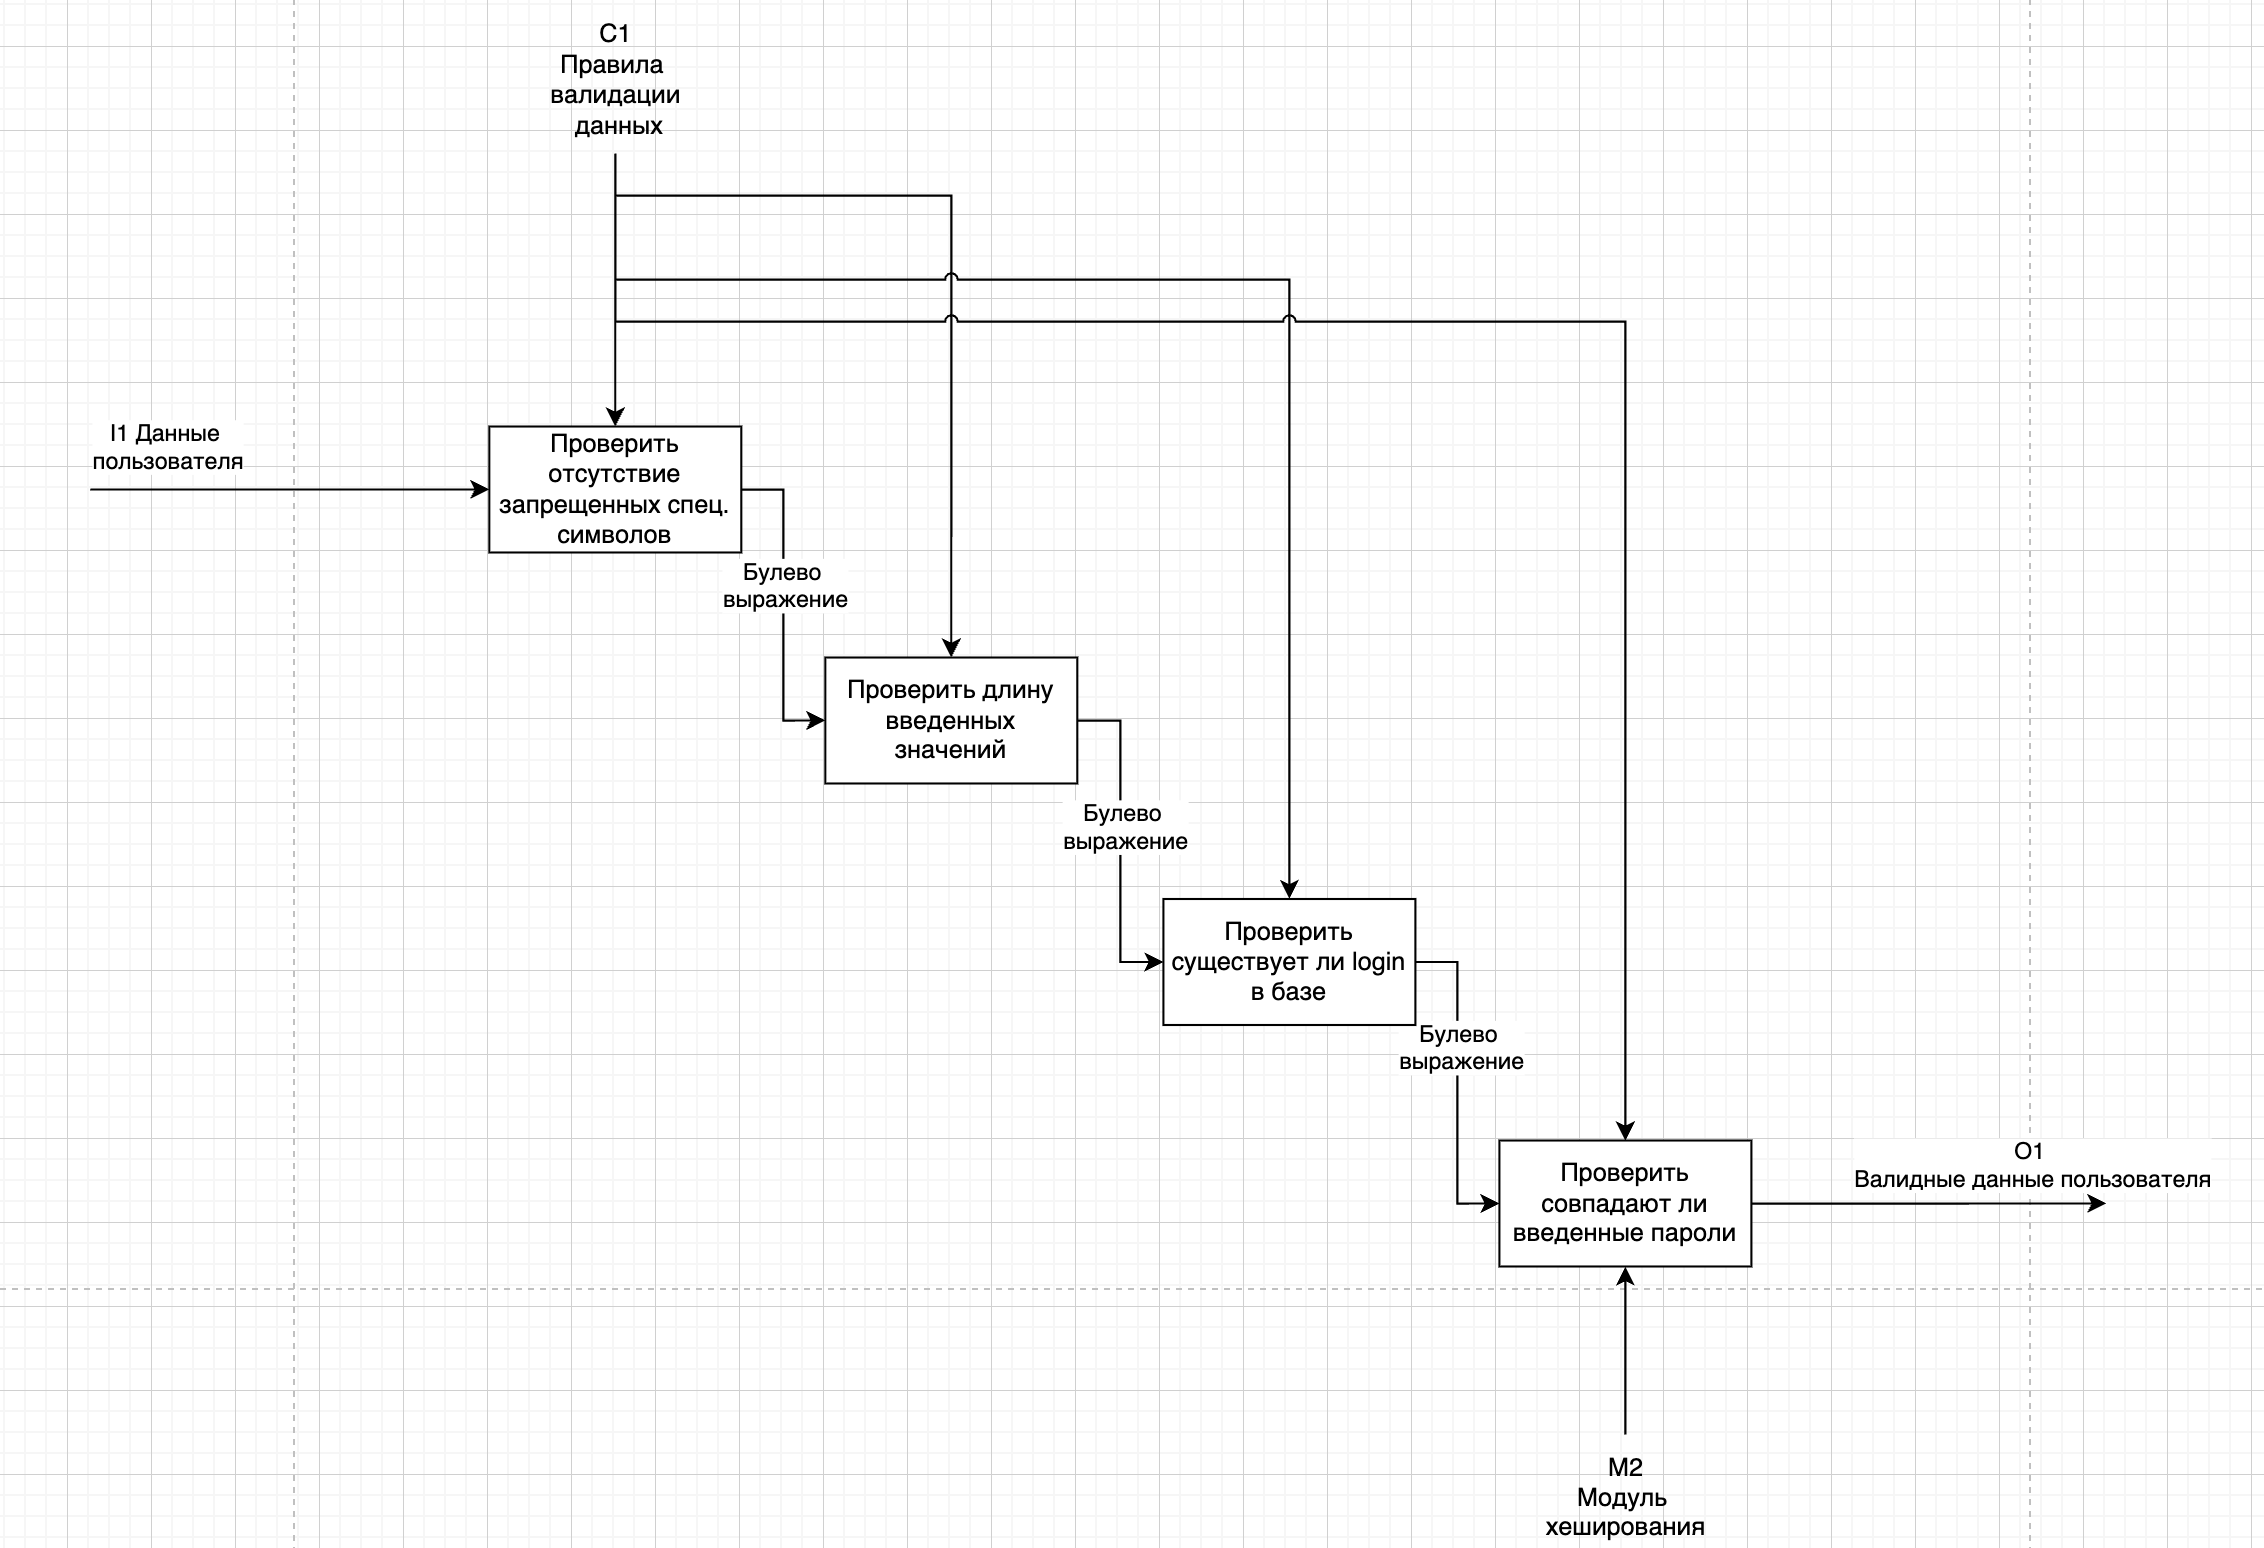
\includegraphics[width=0.7\linewidth]{images/idef0/image4.png}
    \captionof{figure}{Процесс валидации данных в нотации IDEF0.}
    \label{fig:enter-label}
}
Здесь данные сначала валидируется по типу данных (строки числа или другое), далее проверяется существование введенного логина в базе данных, а также сверяются введеные пароли. 

После того как пользователь зарегистрирован, ему необходимо авторизоваться под своим логином для доступа в систему. 

Доступ в систему ограничен специальным токеном авторизации, который пользователь получает по факту авторизации и имеет срок истечения. По истечению срока действия токена, пользователю необходимо заново авторизоваться. ( как правило это очень большой срок и необходимость повторой авторизации возникает при смене браузера или при очистке кеша браузера, поскольку этот токен хранится в локальном хранилище веб сайта).

В процессе авторизации, также используется процесс валидации введенных данных, после чего формируется уникальный идентификатор доступа в систему.

 {
     \centering
     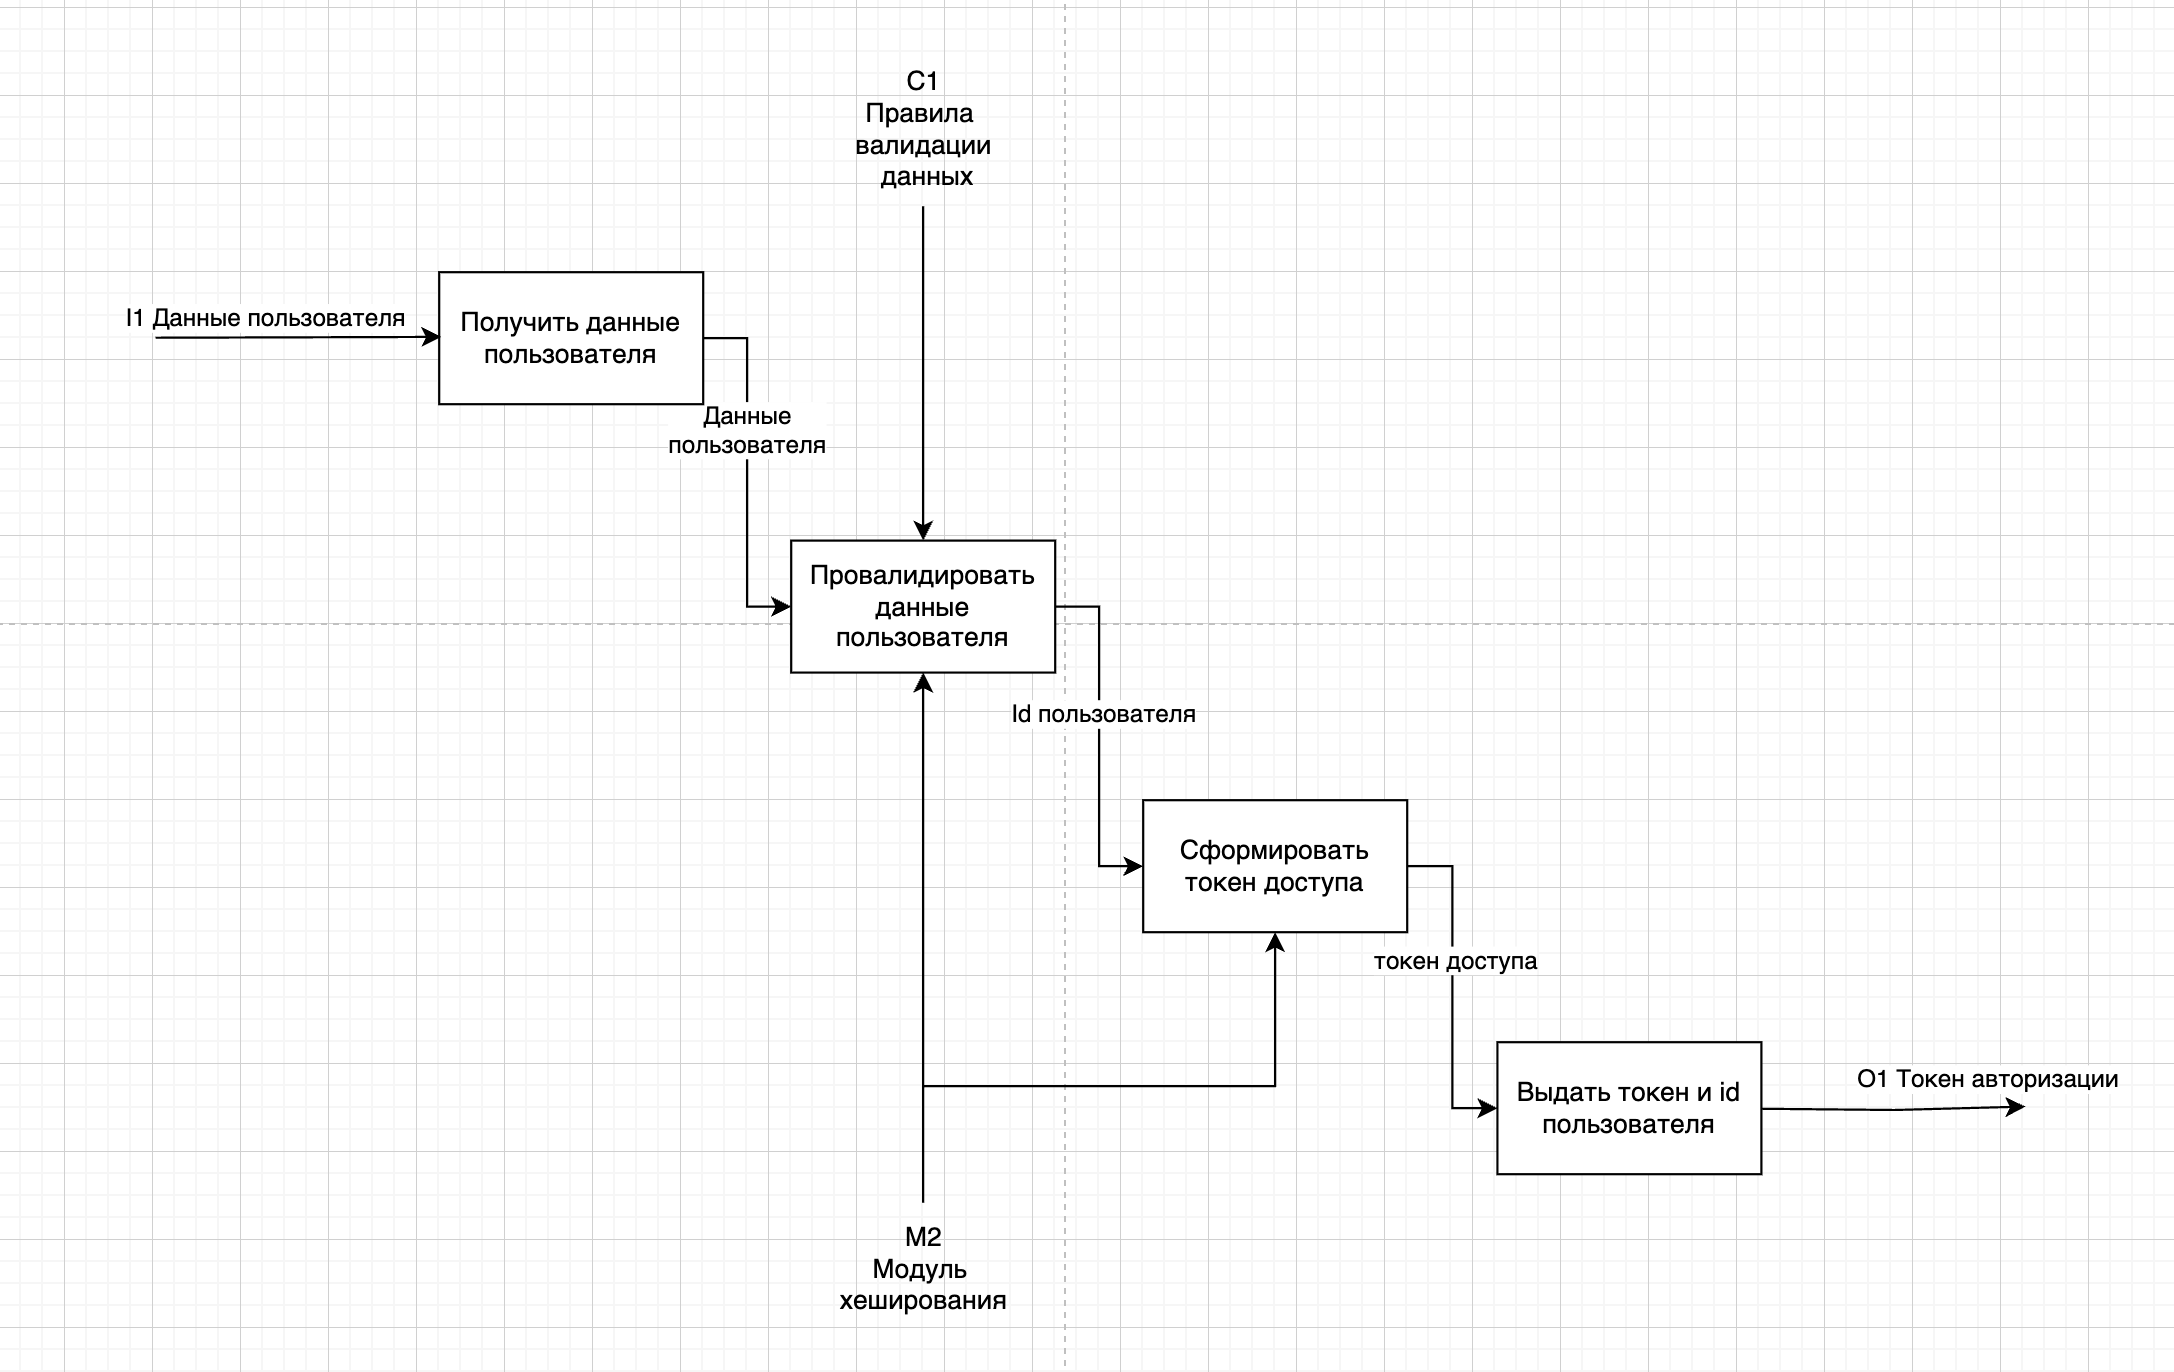
\includegraphics[width=0.7\linewidth]{images/idef0/image5.png}
     \captionof{figure}{Процесс авторизации в нотации IDEF0.}
     \label{fig:enter-label}
 }

\mysubsubsection{Вступление пользователя в группу}

Далее рассмотрим процесс вступления обучающихся в группы. Этот процесс представлен на рисунке 16 в виде диаграммы в нотации BPMN.
{
     \centering
     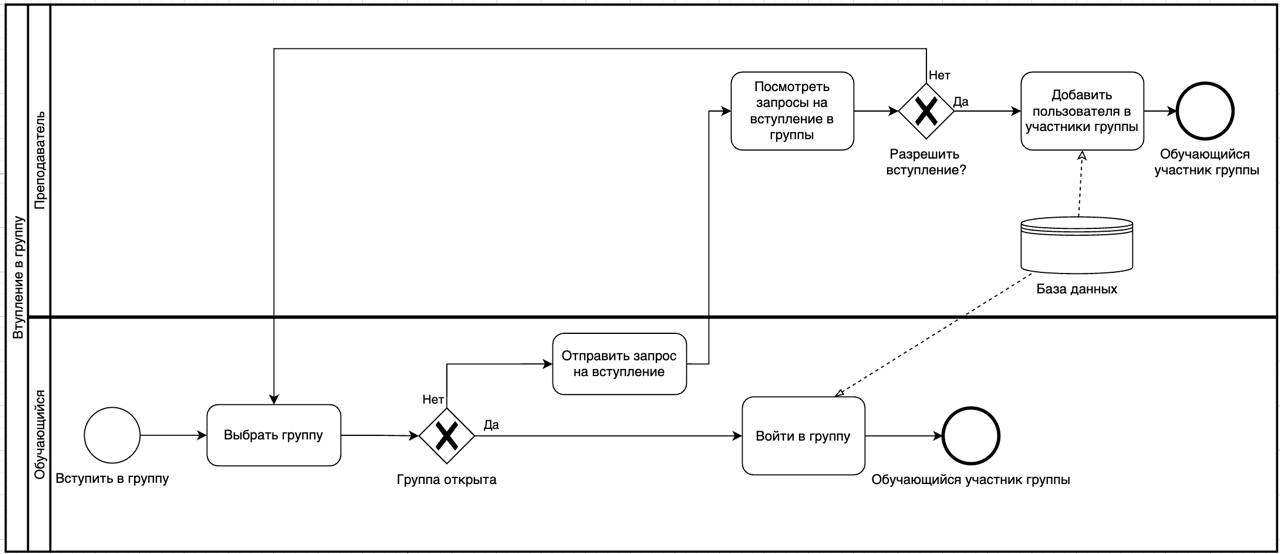
\includegraphics[width=0.7\linewidth]{images/bpmn_grpups.jpg}
     \captionof{figure}{Процесс вступления в группу в нотации BPMN.}
     \label{fig:enter-label}
 }

 Здесь, пользователь, сначала выбирает желаемую группу из списка доступных групп. В случае если группа открыта, то у пользователя есть прямая возможность стать её участником. Этот процесс сопрвождается добавлением новой записи в таблицу участников групп.

 В случае если группа закрыта, создается запрос на вступление в выбранную группу. Создатель этой группы может просмотреть этот запрос и решить, принять участника в группу или нет. Если да, пользователь также добавляется в таблицу участников группы, иначе запрос отклоняется, пользователю предложено выбрать новую группу.

 При этом сам запрос администратор группы не может удалить. Его удалить может только отправитель запроса, в случае если он отзовет заявку на вступление в группу. Администратор также может передумать и спустя время принять заявку на вступление и впустить участника. Но так же может и удалить из группы если его группа изначально была приватна.


\newpage
\mysection{Разработка технической части}

\mysubsection{Анализ техническийх требований}

Для реализации функциональных и нефункциональных требований, необходимо определиться с актуальным стеком технологий. Поскольку итоговым продуктом является веб-приложение, то согласно [источник] современное веб приложение имеет следующие ключевые особенности в разработке:
\begin{enumerate}

\item Отличие в отображении

В отличие от традиционных приложений, веб-приложения функционируют в браузере и предоставляют пользователю взаимодействие с контентом на веб-страницах. Это связано с тем, что веб-приложения базируются на веб-технологиях, таких как HTML, CSS и JavaScript, которые позволяют создавать интерактивные интерфейсы и обеспечивать гибкость в работе с различными устройствами.

\item Раздление компонентов

Веб-приложение как правило состоит из трех основных компонентов: клиентской стороны, серверной стороны и базы данных. Клиентская сторона отвечает за отображение инфорации пользователю и взаимодействие с ним, серверная сторона обрабатывает запросы клиента и принимает решения на основе логики приложения, а база данных хранит и обрабатывает данные, необходимые для работы приложения.

\item Особенности работы

Веб-приложения работают в режиме клиент-серверной архитектуры. Когда пользователь отправляет запрос, браузер обращается к серверу, который обрабатывает запрос и отправляет обратно отображаемые данные. Для этой цели используется протокол HTTP, который обеспечивает передачу данных между браузером и сервером. Таким образом, веб-приложения работают через сеть и доступны пользователю в любом месте, где есть доступ к интернету.


Источник - Школа английского языка Skyeng: https://skyeng.ru/magazine/wiki/it-industriya/chto-takoe-veb-prilozhenie/


Далее в пунктах 2.2 - 2.7 будут рассмотрены все аспекты и компоненты при разработки системы.
\end{enumerate}

\mysubsection{Проектирование базы данных}

В качестве системы управления базой данных я выбрал PostreSQL. 

PostgreSQL - открытая российская система управления базами данных. Она базируется на языке SQL и поддерживает многие из возможностей стандарта SQL:2011 и ряд возможностей SQL:2016 в части работы с данными в формате JSON.

Сильными сторонами PostgreSQL считаются:
\begin{itemize}
    \item высокопроизводительные и надёжные механизмы транзакций и репликации;
    \item расширяемая система встроенных языков программирования: в стандартной поставке поддерживаются PL/pgSQL, PL/Perl, PL/Python и PL/Tcl; дополнительно можно использовать PL/Java, PL/PHP, PL/Py, PL/R, PL/Ruby, PL/Scheme, PL/sh и PL/V8, а также имеется поддержка загрузки модулей расширения на языке C[11];
    \item наследование;
    \item встроенная поддержка слабоструктурированных данных в формате JSON с возможностью их индексации;
    \item расширяемость (возможность создавать новые типы данных, типы индексов, языки программирования, модули расширения, подключать любые внешние источники данных).
\end{itemize}

В PostgreSQL есть следующие ограничения:
\begin{itemize}
    \item максимальный размер таблицы: 32 Тбайт;
    \item максимальный размер поля: 1 Гбайт;
    \item максимум полей в записи: 250—1600, в зависимости от типов полей.
\end{itemize}

На рисунке 17 представлена общая даталогическая модель базы данных. Она включает в себя 12 таблиц и описывает связи между ними.

{
    \centering
    \fbox{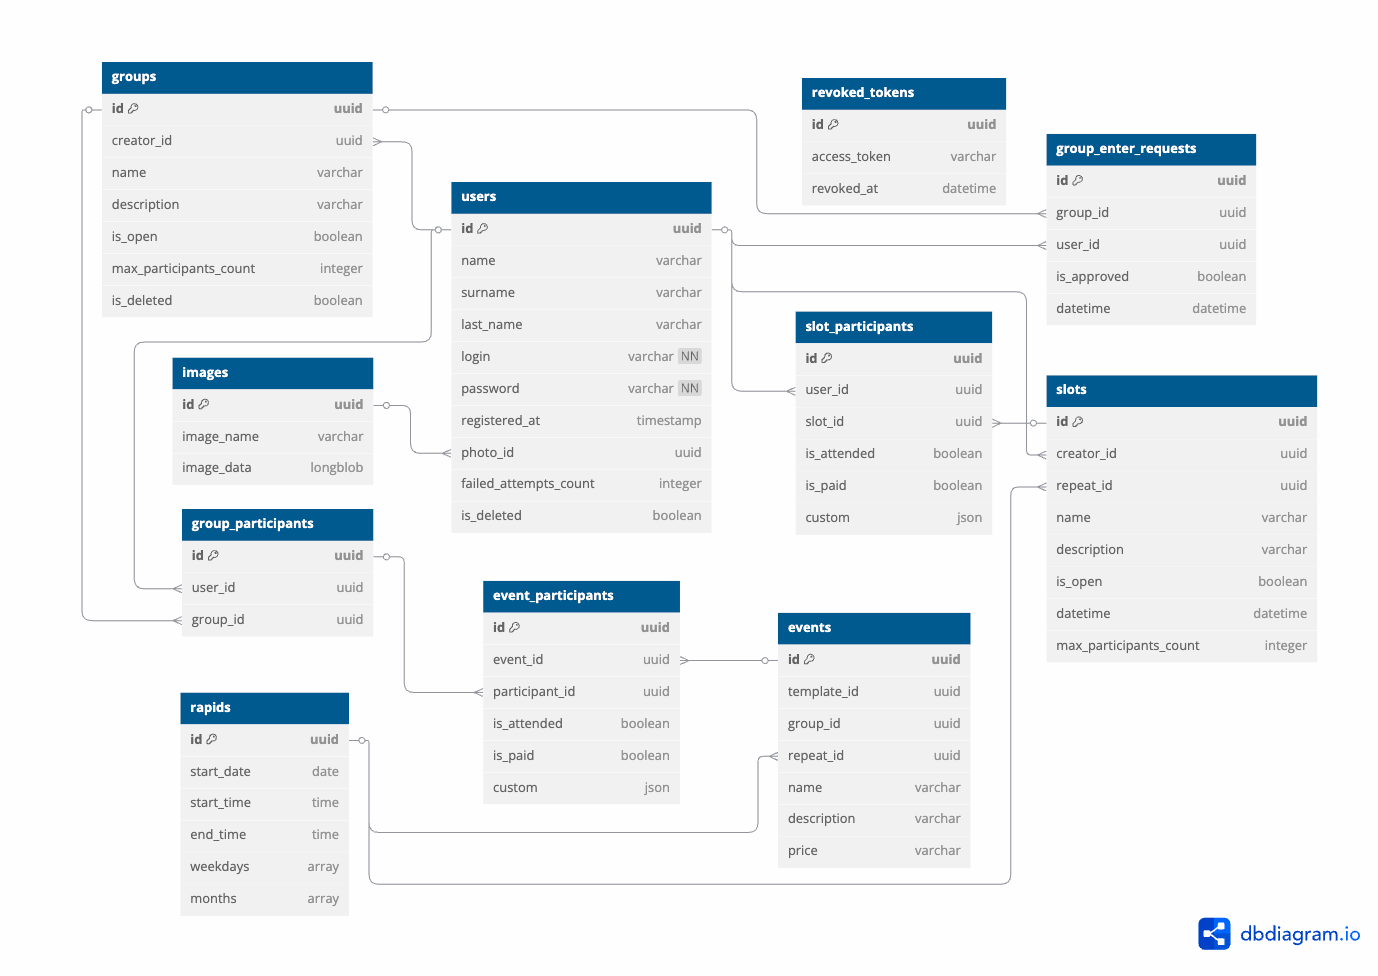
\includegraphics[width=0.5\linewidth]{images/DataBase.png}}
    \captionof{figure}{Схема реляционной базы данных}
    \label{fig:enter-label}
}

\myparagraph{Таблица users}

Содержит информацию о пользователях системы.

\begin{itemize}
    \item login - уникальный логин авторизованного пользователя;
    \item password - хешированный пароль;
    \item photo\_id - идентификатор фотографии;
    \item role\_name - имя роли;
\end{itemize}

\myparagraph{Таблица images}

Содержит информацию об изображениях пользователей.

\begin{itemize}
    \item image\_name - название файла;
    \item image\_data - base64 формат картинки;
\end{itemize}

\myparagraph{Таблица groups}

Содержит информацию о группах - объединения пользователей по общему признаку. Существуют группы открытые как для всех пользователей, так и с ограниченным доступом, за это отвечает поле is\_open.

Все пользователи группы должны присутствовать на всех занятиях, которые создаются управляющим группы.

В открытые могут вступать все желающие, если есть места. 
В закрытые можно вступить, отправив запрос на вступление, который рассмотрит создатель группы.

\begin{itemize}
    \item name - название группы;
    \item max\_participants\_count - максимальное количество участников;
    \item description - описание;
    \item creator\_id - id пользователя, который создал группу
\end{itemize}

\myparagraph{Таблица group\_enter\_requests}

Содержит информацию о запросах пользователей на вступление в закрытые группы.

После принятия пользователя в группу, информация о нем заносится в таблицу group\_participants

\begin{itemize}
    \item user\_id - id пользователя, который отправил запрос;
    \item group\_id - id группы, в которую пользователь хочет вступить;
    \item datetime - дата и время создания запроса.
    \item is\_approved - флаг о принятом или отклоненном запросе. 
    
    Его состояния: 
        \begin{itemize}
            \item null - запрос еще не рассмотрен;
            \item False - запрос не удовлетворен.
            \item True - запрос удовлетворен и пользователь заносится в таблицу участников;
        \end{itemize}
\end{itemize}


\myparagraph{Таблица group\_participants}

Содержит информацию о группах и пользователях, для определения кто в какой группе состоит или не состоит.
Пользователи могут состоять в сразу нескольких группах.

\begin{itemize}
    \item group\_id - уникальный идентификатор группы; 
    \item user\_id - уникальный идентификатор пользователя.
\end{itemize}

\myparagraph{Таблица events\_template}
Содержит информацию о шаблонах событий. Являются шаблонами события или одного занятия, которое создает создатель группы. Он указывает описание и название занятия и частоту повторения.

\begin{itemize}
    \item group\_id - группа, в которой это событие происходит
    \item repeat\_id - ссылка на таблицу \texttt{rapids} с указанием частоты
\end{itemize}

\myparagraph{Таблица events}

Содержит информацию о частных событиях, которые являются "наследниками" \texttt{events\_templates}. 
Частные события создаются в момент начала занятия администратором группы. Когда администратор видит в интерфейсе, что у него по расписанию сейчас должно начаться занятие, он нажимает кнопку - создается конкретное занятие.
\begin{itemize}
    \item datetime - дата и время, в которое проходит конкретно это событие
\end{itemize}


\myparagraph{Таблица group\_event\_participants}


Информация об участниках одного конкретного события .

О каждом участнике ведется следующая информация: его присутствие, оплачата занятия, а также другие индивидуальные параметры.

\myparagraph{Таблица slots}

Содержит ифнормацию об открытых занятиях вне групп. Их назначение схоже с назначением событий, но отсутствует слой с группами. Каждый слот - является одновременно и группой, и занятием.

Пользователи могут вступить в открытый слот. В закрытый - только по приглашению создателя. У слота указана частота повторения.

\myparagraph{Таблица slot\_participants}

Содержит информацию об участниках открытых событий.

Идет лишь ссылка по slot\_id к slots чтобы указать наследник какого слота эта запись.
    

\mysubsection{Описание и разработка необходимых компонентов системы}

Сегодня серверные компоненты веб приложений реализуют множеством различных способом, с использованием различных языков программирования. Самые популярные из них:
\begin{itemize}
    \item PHP
        \begin{itemize}
            \item[+] Огромное наследие, множество готовых решений (WordPress, Laravel).
            \item[+] Низкий порог входа.
            \item[+] Хорошая документация.
            \item[-] Устаревшая архитектура во многих проектах.
            \item[-] Проблемы с производительностью в высоконагруженных системах.
            \item[-] Нестрогая типизация.
        \end{itemize}
    \item Go
        \begin{itemize}
            \item[+] Высокая производительность.
            \item[+] Простая конкурентная модель (горутины).
            \item[+] Статическая компиляция.
            \item[-] Меньше библиотек по сравнению с Python/Node.js.
            \item[-] Строгий синтаксис (меньше гибкости).
            \item[-] Слабее в быстрой разработке прототипов.
        \end{itemize}
    \item Node JS
        \begin{itemize}
            \item[+] Асинхронная модель из коробки
            \item[+] Один язык для frontend и backend
            \item[+] Большая экосистема (npm)
            \item[-] Callback hell (хотя есть async/await)
            \item[-] Слабая типизация (TypeScript решает частично)
            \item[-] Проблемы с CPU-интенсивными задачами
        \end{itemize}
    \item Python
        \begin{itemize}
            \item[+] Читаемый и выразительный синтаксис
            \item[+] Богатейшая экосистема (Django, Flask, FastAPI)
            \item[+] Лучший выбор для AI/Data Science
            \item[-] GIL ограничивает многопоточность
            \item[-] Медленнее компилируемых языков
            \item[-] Динамическая типизация (но есть type hints)
        \end{itemize}
\end{itemize}

В качестве основного языка программирования выбран Python. Для создания функционального веб сервиса выбран фреймворк FastAPI.
Выбор обусловлен следующими факторами:
\begin{itemize}
    \item Быстрая разработка: Python позволяет быстро создавать прототипы
    \item Современный подход: FastAPI предоставляет:
    \begin{itemize}
        \item Автоматическую документацию (OpenAPI/Swagger)
        \item Встроенную валидацию через Pydantic
        \item Поддержку async/await
    \end{itemize}
    \item Гибкость: Возможность интеграции с:
    \begin{itemize}
        \item ML-моделями
        \item Аналитическими инструментами
        \item Внешними сервисами
    \end{itemize}
    \item Сообщество: Огромное количество готовых решений и библиотек
    \item Производительность: FastAPI сравним по скорости с Node.js и Go в типичных web-задачах
\end{itemize}

Python + FastAPI — оптимальный баланс между скоростью разработки,\\производительностью и поддерживаемостью кода для учебного проекта.

\mysubsubsection{Движение данных от клиента к серверу}
Определившись с стеком технологий, рассмотрим архитектуру серверной части приложения. На рисунке \_ представлена MVC схема движения данных внутри сервера.


{
    \centering
    \fbox{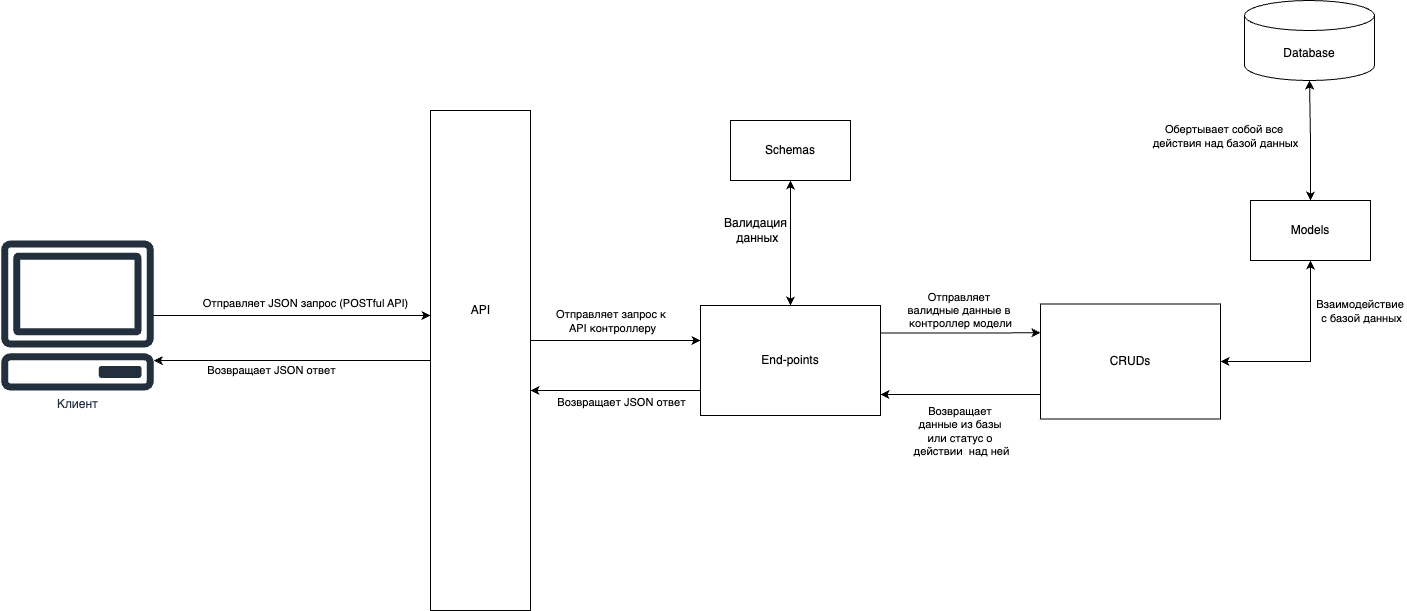
\includegraphics[width=0.7\linewidth]{images/Diploma-Слои backend.png}}
    \captionof{figure}{Схема взаимодействия данных от клиента до базы данных}
    \label{fig:enter-label}
}

С клиента поступает JSON запрос на получение, изменение, удаление или создание определенных данных.

По указанному API выполняется определнный END-поинт - точка входа в клиентское приложение.
Прежде чем работать с данными - их необходимо отвалидировать, проверить, что данные удовлетворяют требованиям схем. За это отвечают схемы валидации - Schemas на диаграмме. 

В зависимости от ендпоинта выполняется бизнес логика взаимодействия с базой данных CRUD - акроним от Create Read Update Delete. В крудах происходит непосредственное взаимодействие с моделями. Модель - ORM представление таблицы в базе данных, обеспечивающая упрощенный доступ к взаимодействию с данными. В отличии от схемы, модель позволяет не только дополнительно отвалидировать данные, но предоставляпт функционал к генерации SQL запросов к базе данных.

Полученные данные из базы, дополнительно форматируются на уровне крудов, для необходимого формата чтения данных клиентской частью и передаются обратно в контроллер API - ендпоинт. Здесь происходит повторная валидация с помозью схем, чтобы удостовериться, что полученные данные из круда являются ожидаемым форматом для фронт-енд части. 

После чего ендпоинт возвращает JSON ответ на клиент.

\mysubsubsection{Используемые модули для обеспечения внутреннего взаимодействия}

Идеальным ORM поставщиком является sqlAlchemy - позволяет использовать модельный архитектурный подход, в котором каждая таблица в базе данных представлена моделью с которой работает система. Это позволяет не использовать чистый SQL, а оперировать встроенным функционалом запросов, методы query для составления сложных SQL запросов. 

На слое валидации я использую схемы от модуля Pydentic. Этот модуль позволяет не описывать входные и выходные параметры в yaml файлах, вся валидация происходит в специальных классах - схемах где указываются типы полей и pydentic схема сама валидирует введенные и возвращаемый параметры данных. Зачастую они схожи с sqlAlchemy моделями и поэтому их описание занимает гораздо меньше времени.

В качестве системы контроля версий был выбран github.

В качестве системы запуска приложения выбрал Docker контейнеры, обеспечивающие быстрый запуск приложения в режиме разработки и выпуска финальной версии продукта. Достаточно описать команды для деплоя докер контейнеры, так все необходимые файлы попадут в контейнер.
\mysubsection{Описание вспомогательных компонентов для взаимодействия по HTTP}

Как я упоминал ранее, на уровне API, первой точкой входа в систему это end-поинты. Они являются публичными методами, которые использует фронтенд часть проекта.

Для оптимизации временных затрат я принял решение использовать POSTful API для того, чтобы не разделять логику процессов на риазличные типы запросов. Любое получение, изменение и создание сущностей в базе данных происходит через POST запросы. Они имеют закрытый body в формате JSON, обеспечивая поддержку любого типа данных ( будь это строки, числа, массивы или объекты)

В папке endpoints у меня лежат все файлы относящиеся к сущностям. Например, enter\_requests модуль отвечает за создание, чтение, удаление, а также за принятие и отклонение запросов на вступление в закрыте группы пользователей. 

Однако, с увеличением количества отдельных модулей возникает необходимость в оптимизации процесса добавления этих модулей в \_\_init\_\_ файл. Этот файл позволяет использовать все внутренниие файлы папки как один модуль, просто ссылаясь на папк endpoints. 

Для того чтобы избежать ручной ввод путей в этот инит файл, а также чтобы отловить все возможные ошибки внутри ендпоинтов и крудов, которые используются внутри них и не дать приложению не запуститься в принципе, я разрботал алгоритм, интегрирующий роутеры каждого ендпоинта в один общий роутер используемый FastAPi приложением. Этот алгоритм представлен на листинге 1.

\begin{lstlisting}[language=Python, caption=Алгоритм сбора маршрутов,breaklines=true, numbers=left]
"""
Entry point for all endpoints
"""

import os
import importlib
from fastapi import APIRouter
from env_constants import BASE_URL

app_router = APIRouter()


def include_routers(app_router: APIRouter):
    endpoints_path = os.path.join(os.path.dirname(__file__), 'endpoints')
    for filename in os.listdir(endpoints_path):
        if filename.endswith('.py') and filename != '__init__.py':
            module_name = filename[:-3]
            try:
                module = importlib.import_module(
                    f'api.endpoints.{module_name}')
                if hasattr(module, 'router'):
                    app_router.include_router(
                        module.router, prefix=f'/{BASE_URL}', tags=[module_name])
                    print(f'{module} router is added')
            except Exception as e:
                print(f'Failed to include router from {filename}: {e}')


include_routers(app_router)

\end{lstlisting}

Разберемся более детально в происходящем:

Перед тем как вызвать функцию агрегации маршрутов API я создаю общий FASTApi роутер в который буду добавлять все роутеры из модулей в папке edpoints.

Первым делом получаю абсолютный путь к папке в которой хранятся все наши ендпоинты (папка edpoints) с помощью встроенной библиотеки os (строка 14)

Далее итерируюсь по списку файлов внутри директории ендпоинтов (строка 15)

В случае если имя файла содержит \_\_init\_\_ - пропускаю этот файл и двигаюсь дальше (строка 16)

Далее с помощью бибилотеки importlib я динамически загружаю содержимое файла в оперативную память (строка 19). В случае если в модуле содержится переменная router, я включаю его в свой общий роутер. Таким образом, область включения маршрутов включает в себя все существующие маршруты без необходимости вручную импортировать их в общий инит файл.

Далее, в случае если один из роутеров содержит в себе ошибку, сработает обработчик Exception (строка 25) и выведет в консоль трейс ошибки и причину по которой маршрут не смог собраться. 

Далее в приложении уже используется обще собранный роутер со всеми рутами к ендпоинтам.
% \mysubsection {Юнит-тестирование}
\mysubsection{Разработка интерфейса}

На рисунке 18 представлен макет страницы для входа в систему. Это форма с двумя полями, у каждого поля для ввода есть подсказки, а также указаны ошибки если введенные значения некорректны. Также, поле для ввода имеет глазик для предпосмотра введенного пароля.

{
    \centering
    \fbox{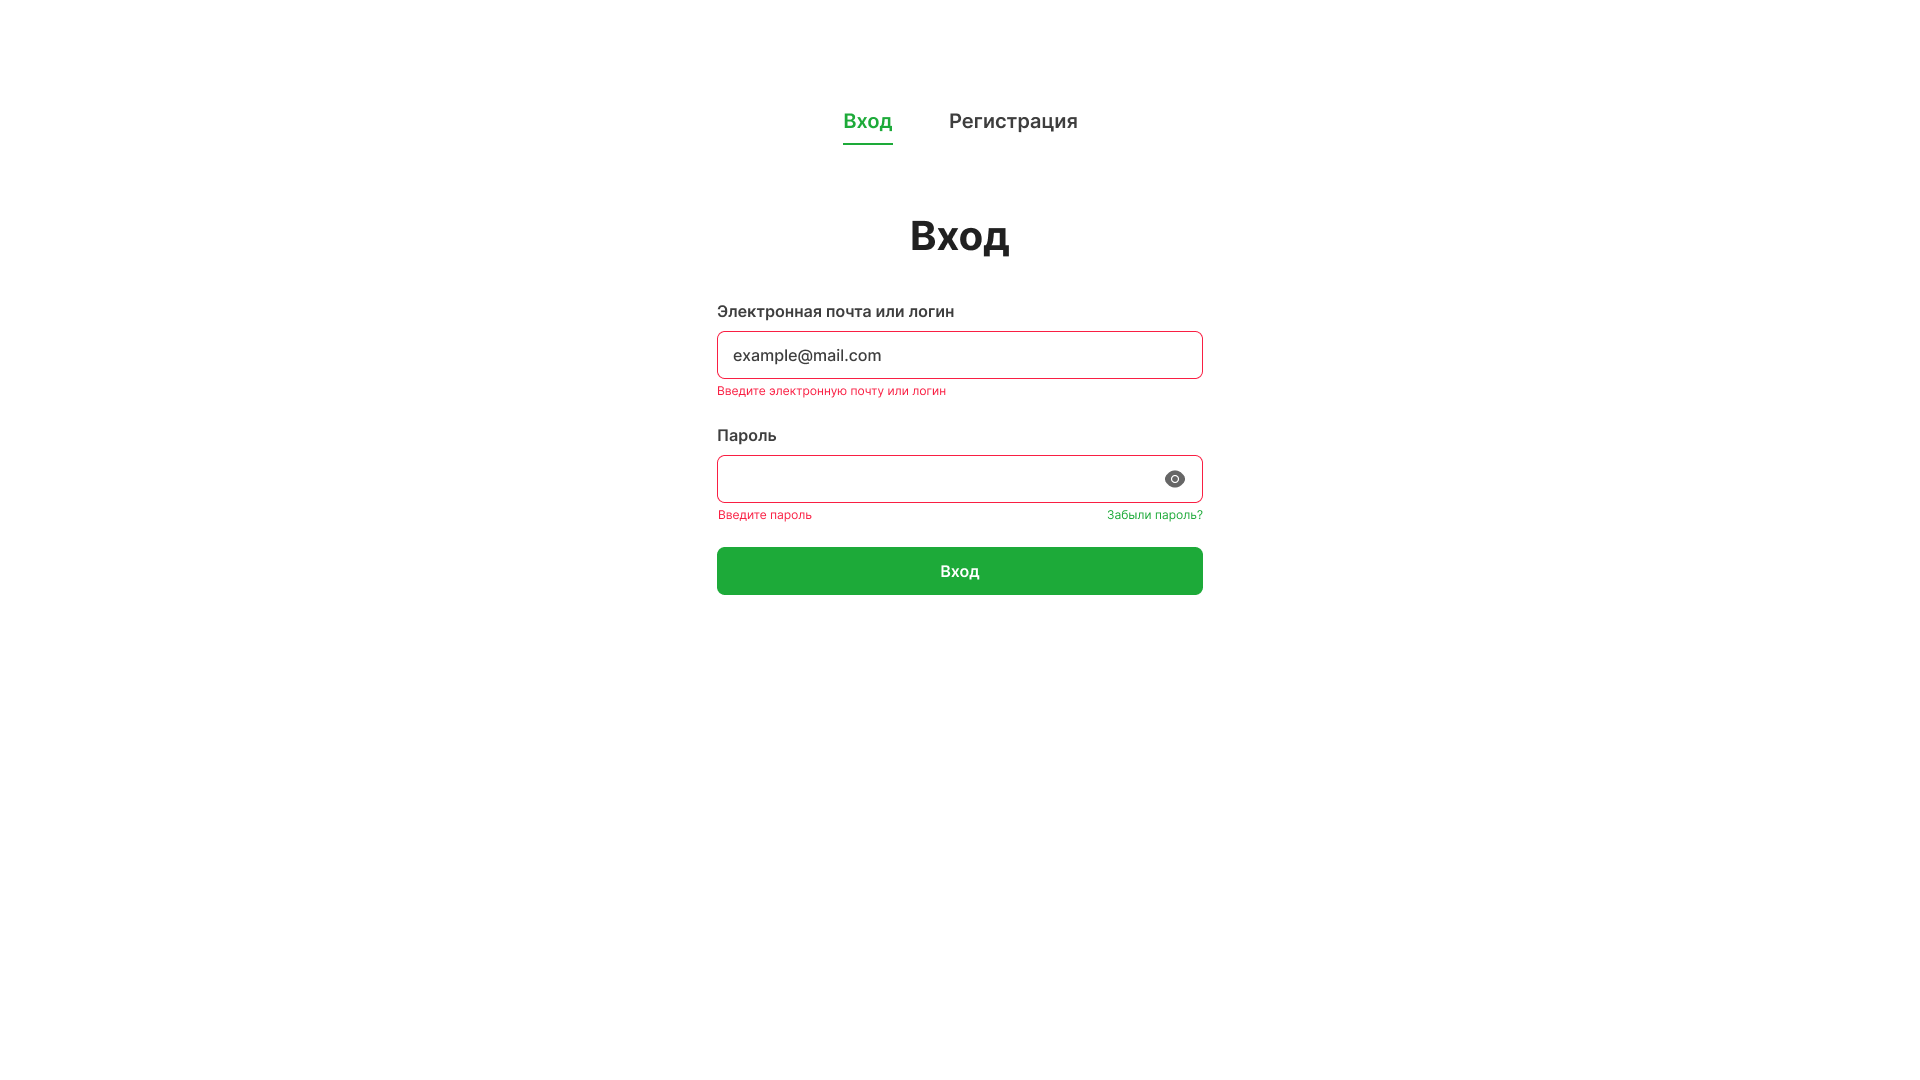
\includegraphics[width=0.7\linewidth]{images/design/Вход.png}}
    \captionof{figure}{Прототип страницы Вход}
    \label{fig:enter-label}
}

На рисунке 19 представлен макет страницы для регистарции в системе. В форме представлены основные поля необходимые лдя регистрации нового пользователя. При вводненесовпадающих пароей, высвечивается соответствующее сообщение о валидации. Также, под кнопкной о регистрации можно найти ссылку на условия обработки персональных данных.

{
    \centering
    \fbox{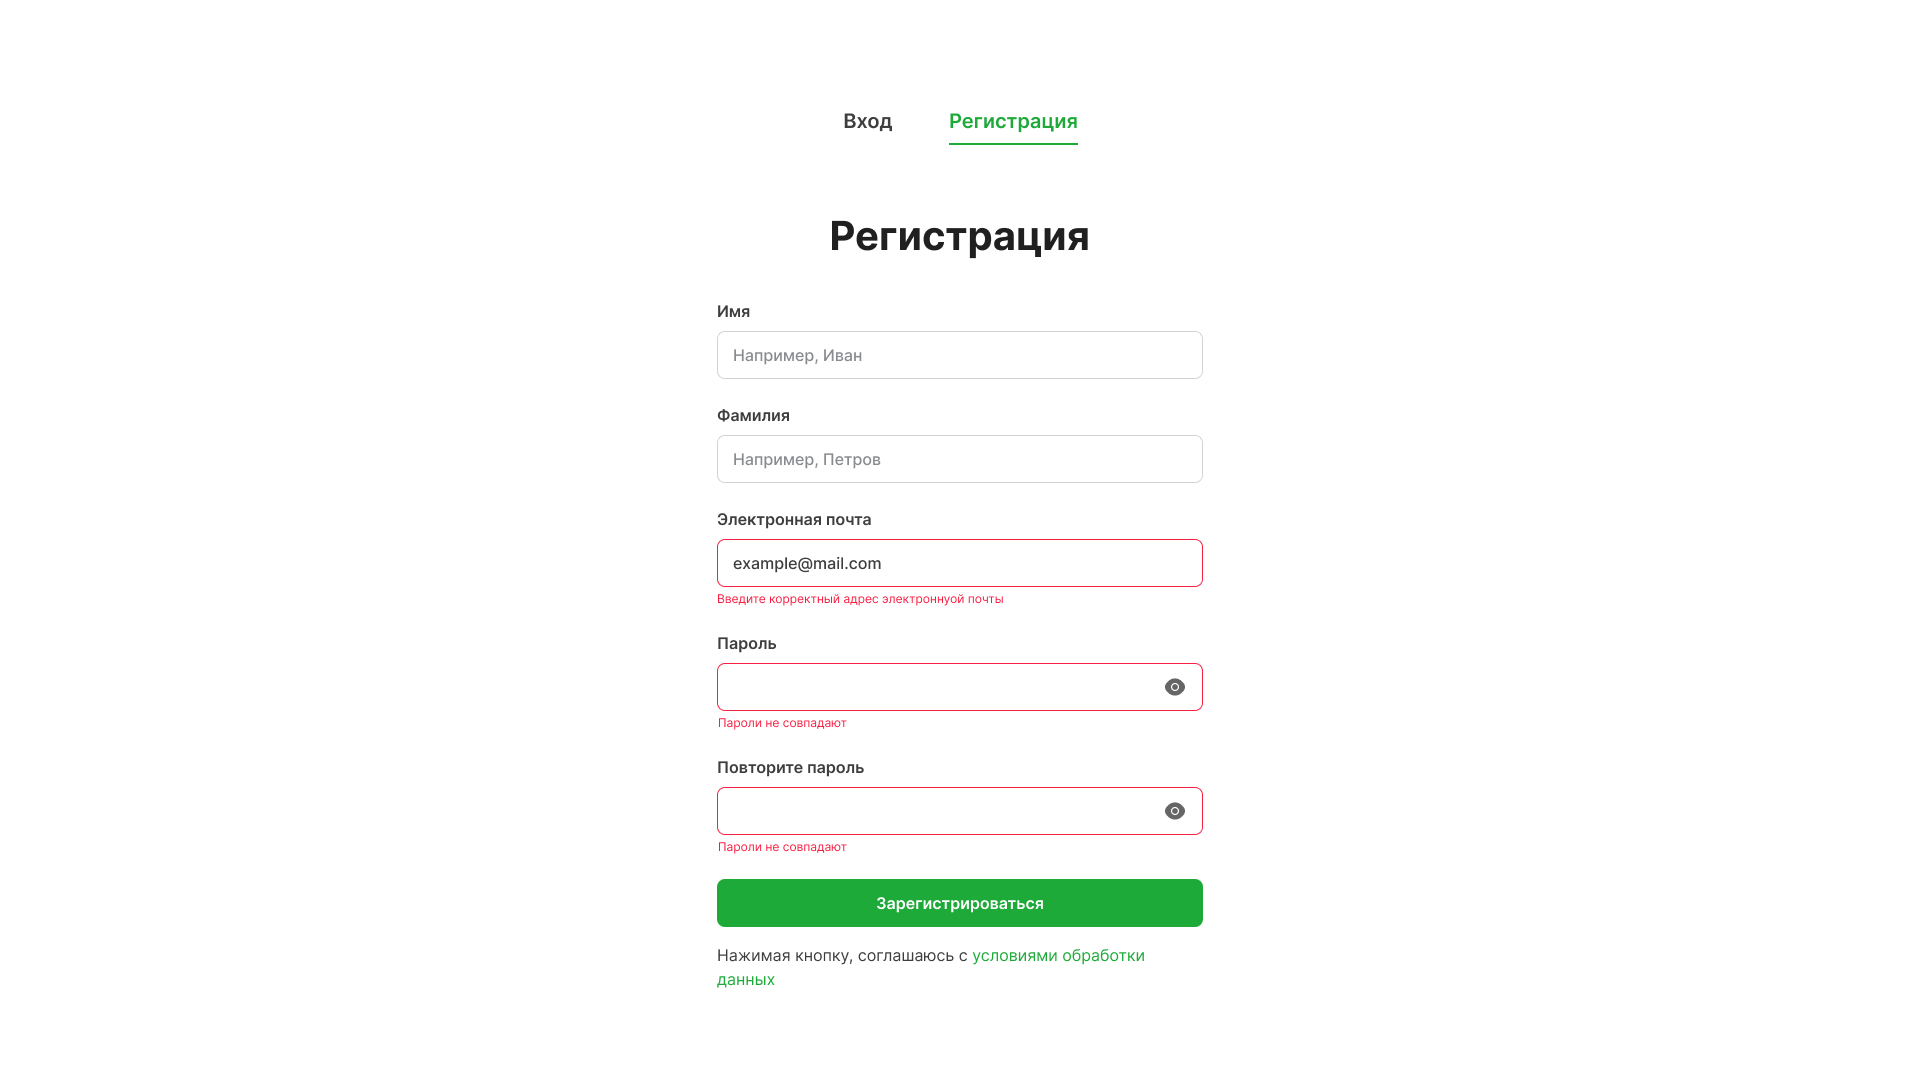
\includegraphics[width=0.7\linewidth]{images/design/Регистрация.png}}
    \captionof{figure}{Прототип страницы Регистрация}
    \label{fig:enter-label}
}

На рисунке 20 представлен макет страницы расписания пользователя - одного из 3 основных разделов сервиса. На вкладке расписание находится интерактивный компонент с календарем, позволяющий переключаться между месяцами, а также кнопкой создания занятия на выбранную дату. 

Справа от него находится более подробный компонент календаря с переключением между днем (рисунок 20), неделей (рисунок 21) и месяцем (рисунок 22). 

В каждом из них в удобном формате представлены предстоящие занятия среди всех групп.
\newpage
{
    \centering
    \fbox{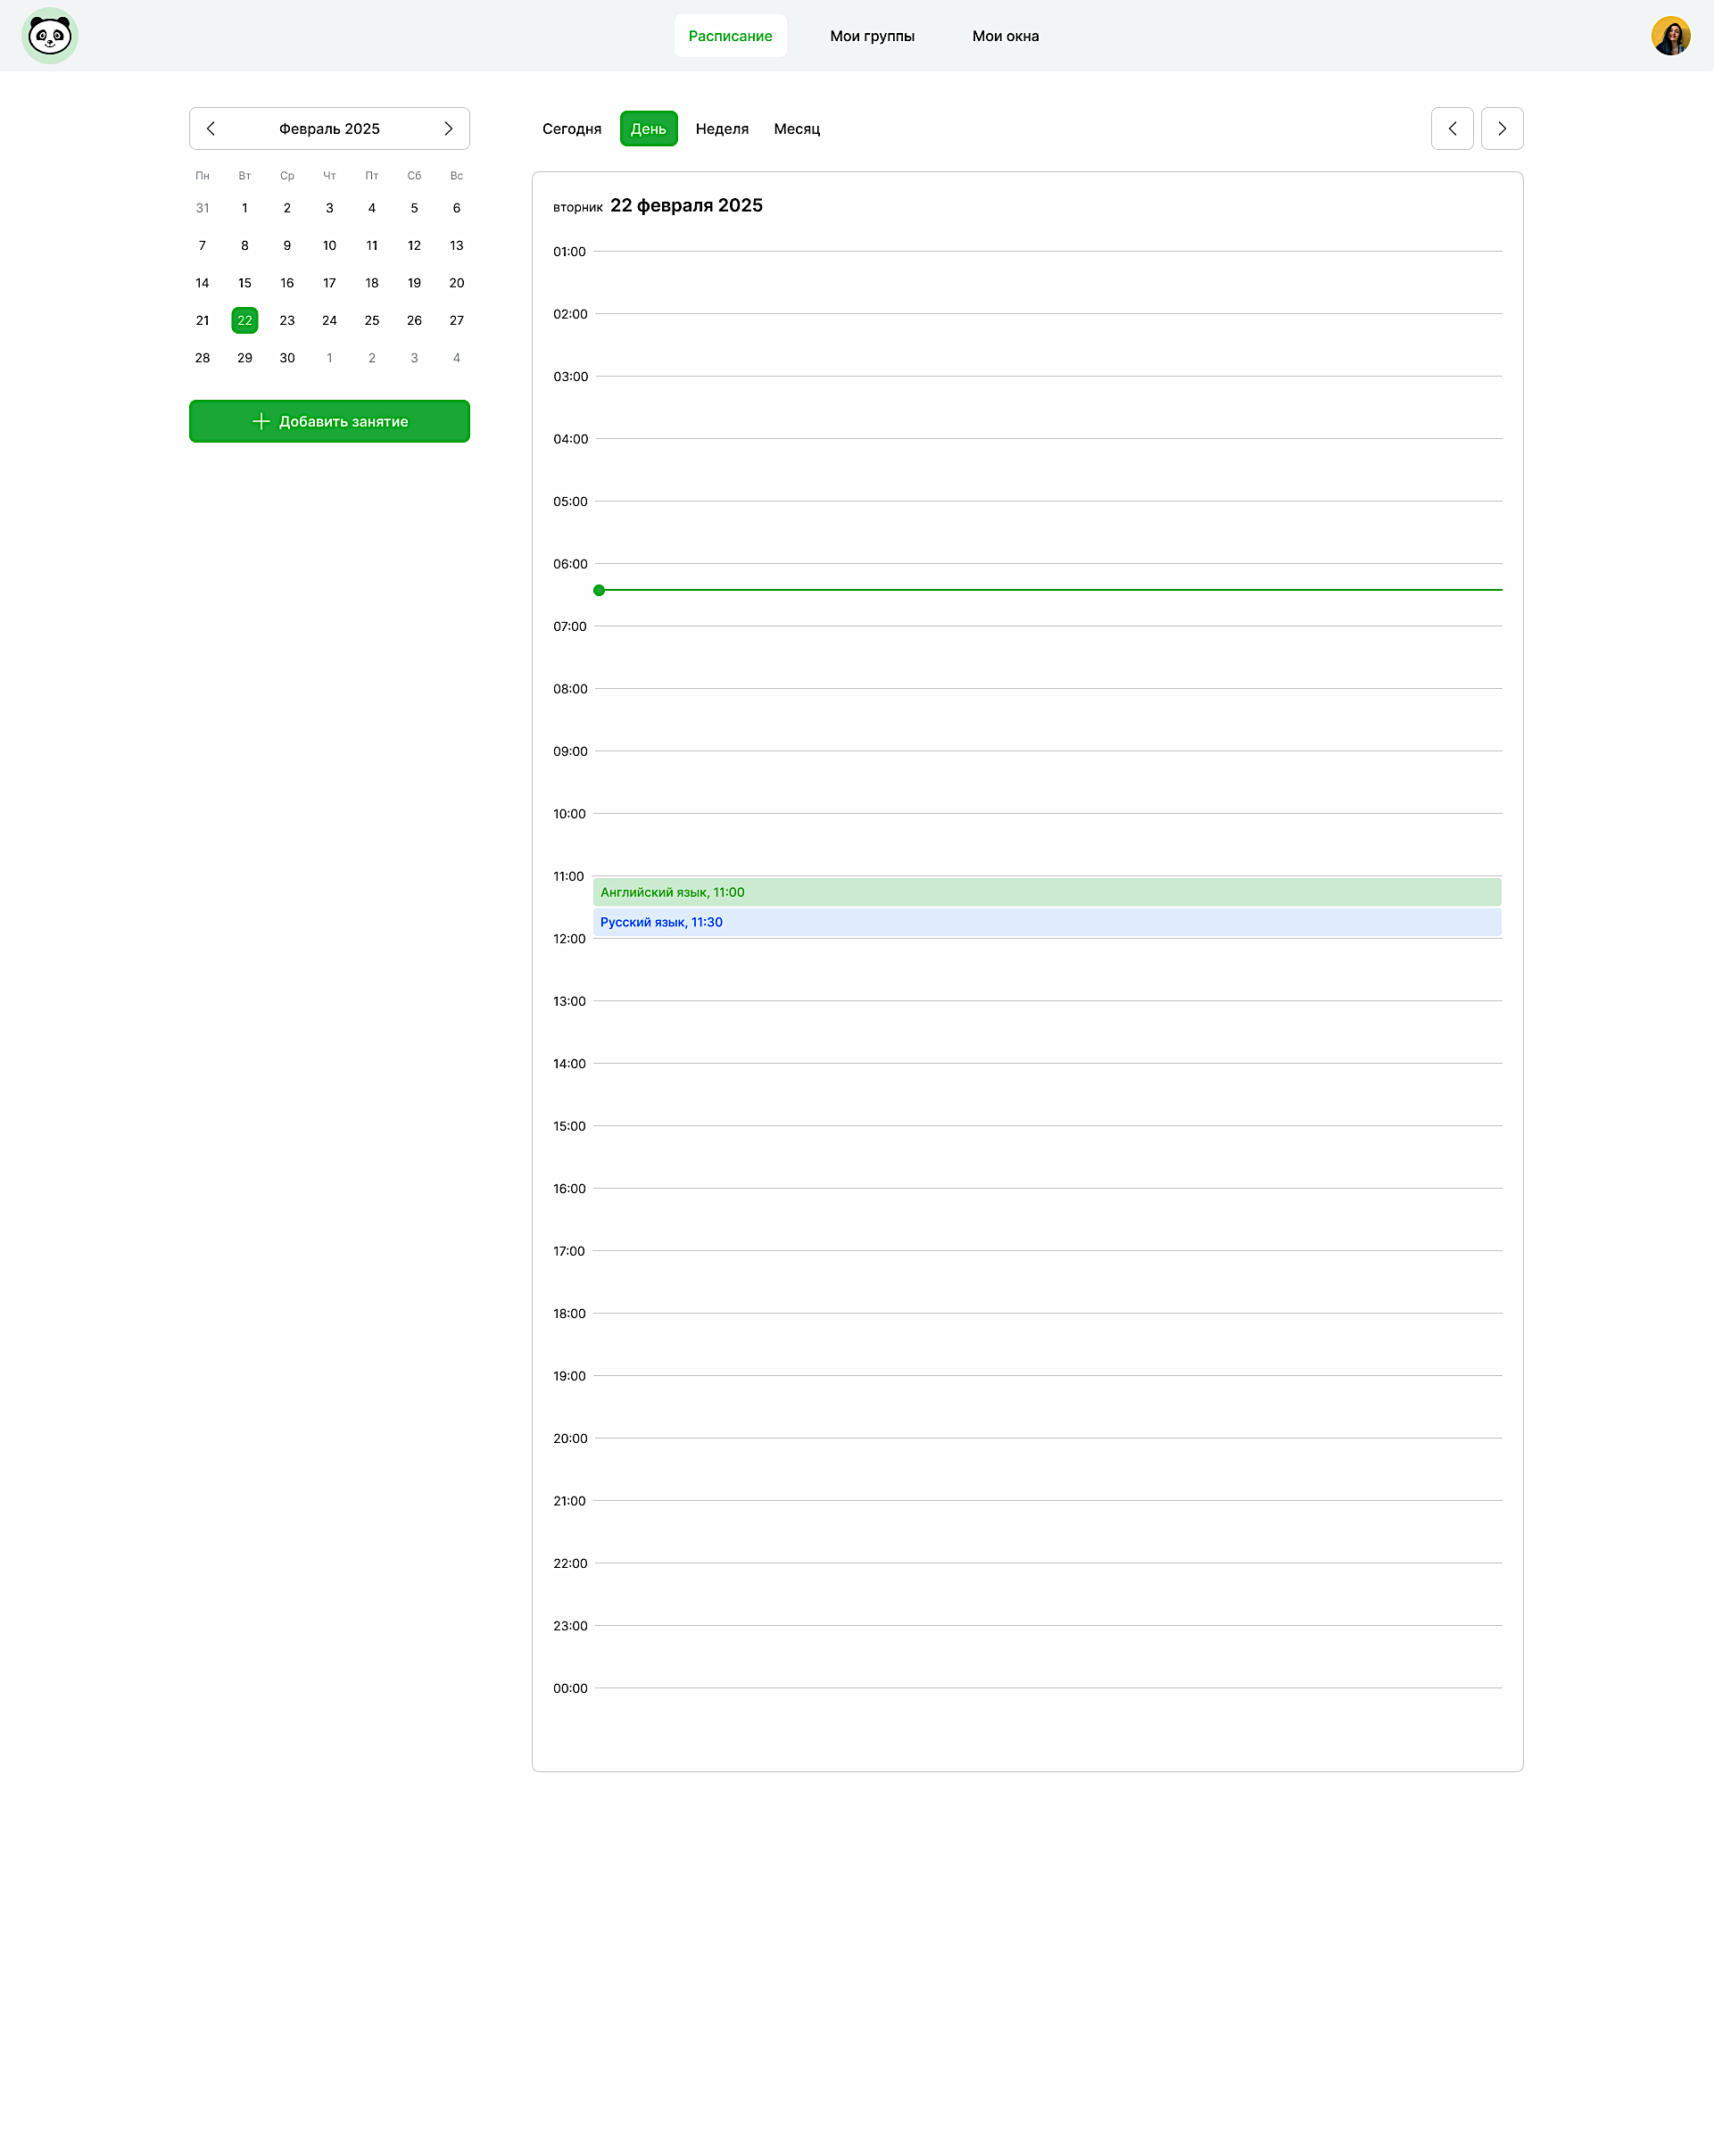
\includegraphics[width=0.7\linewidth]{images/design/Расписание_День.png}}
    \captionof{figure}{Прототип страницы "Расписание". Календарь, день}
    \label{fig:enter-label}
}


{
    \centering
    \fbox{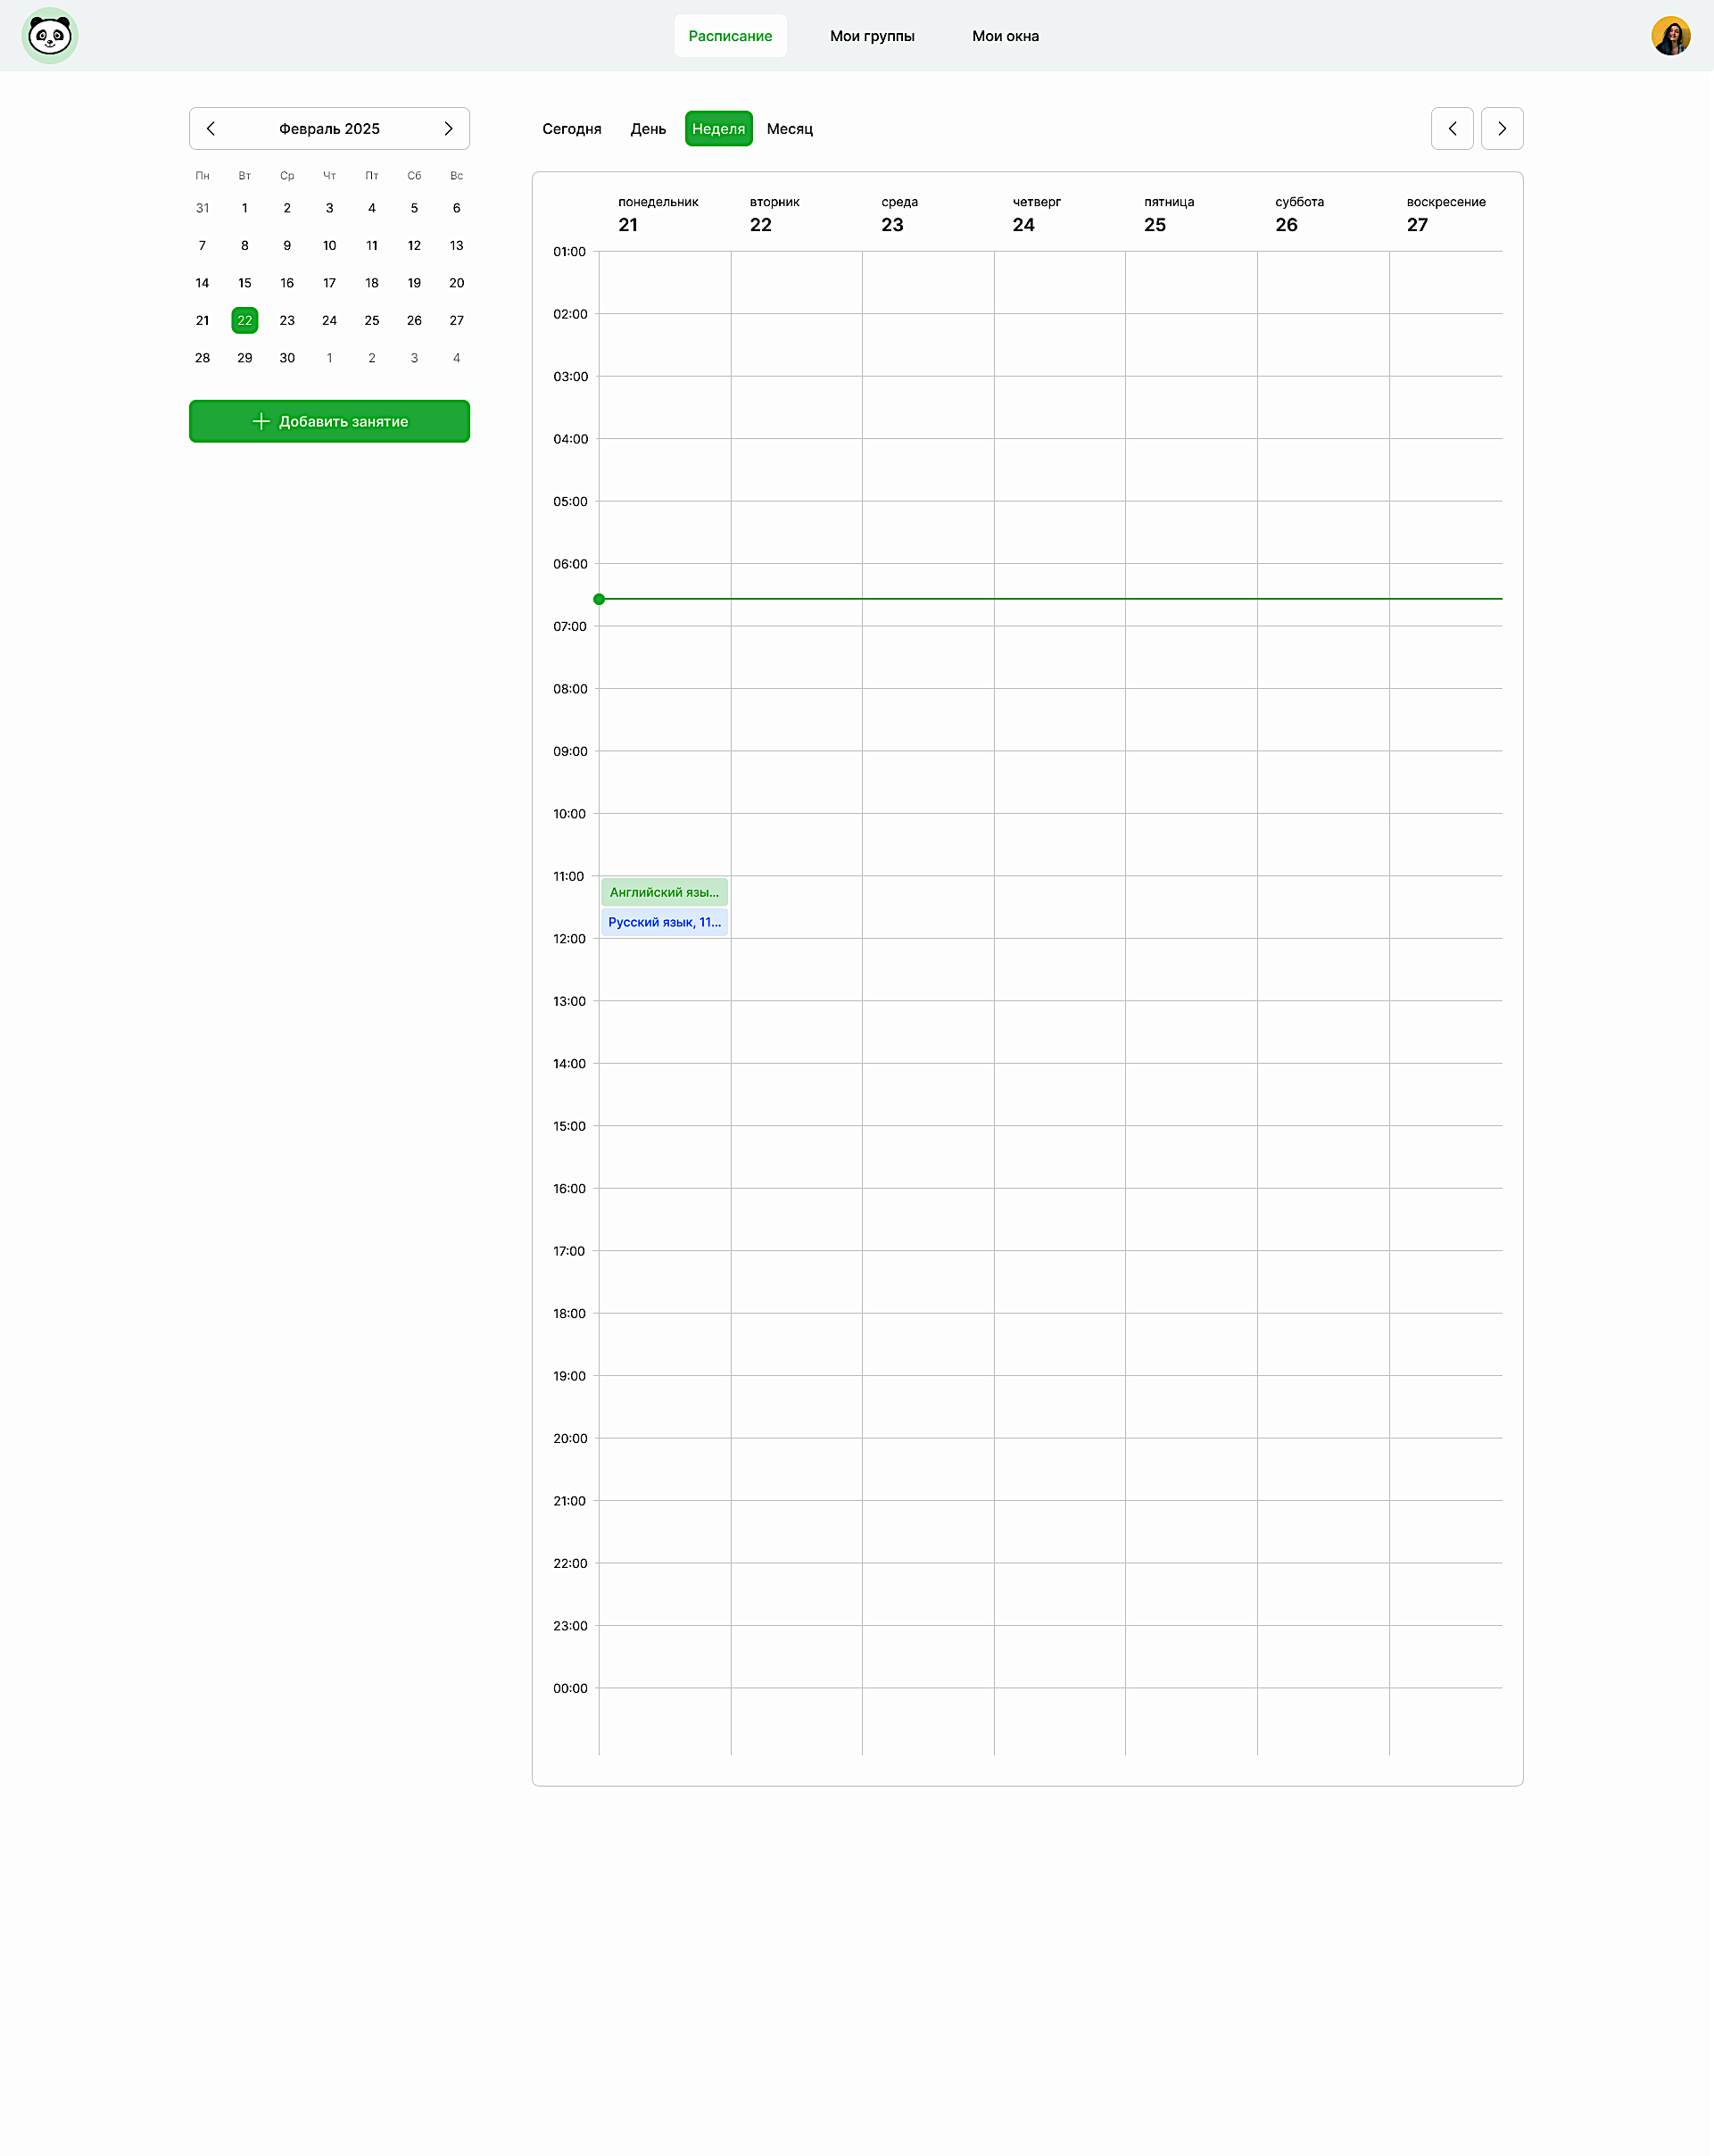
\includegraphics[width=0.5\linewidth]{images/design/Расписание_Неделя.png}}
    \captionof{figure}{Прототип страницы "Расписание". Календарь, неделя}
    \label{fig:enter-label}
}

{
    \centering
    \fbox{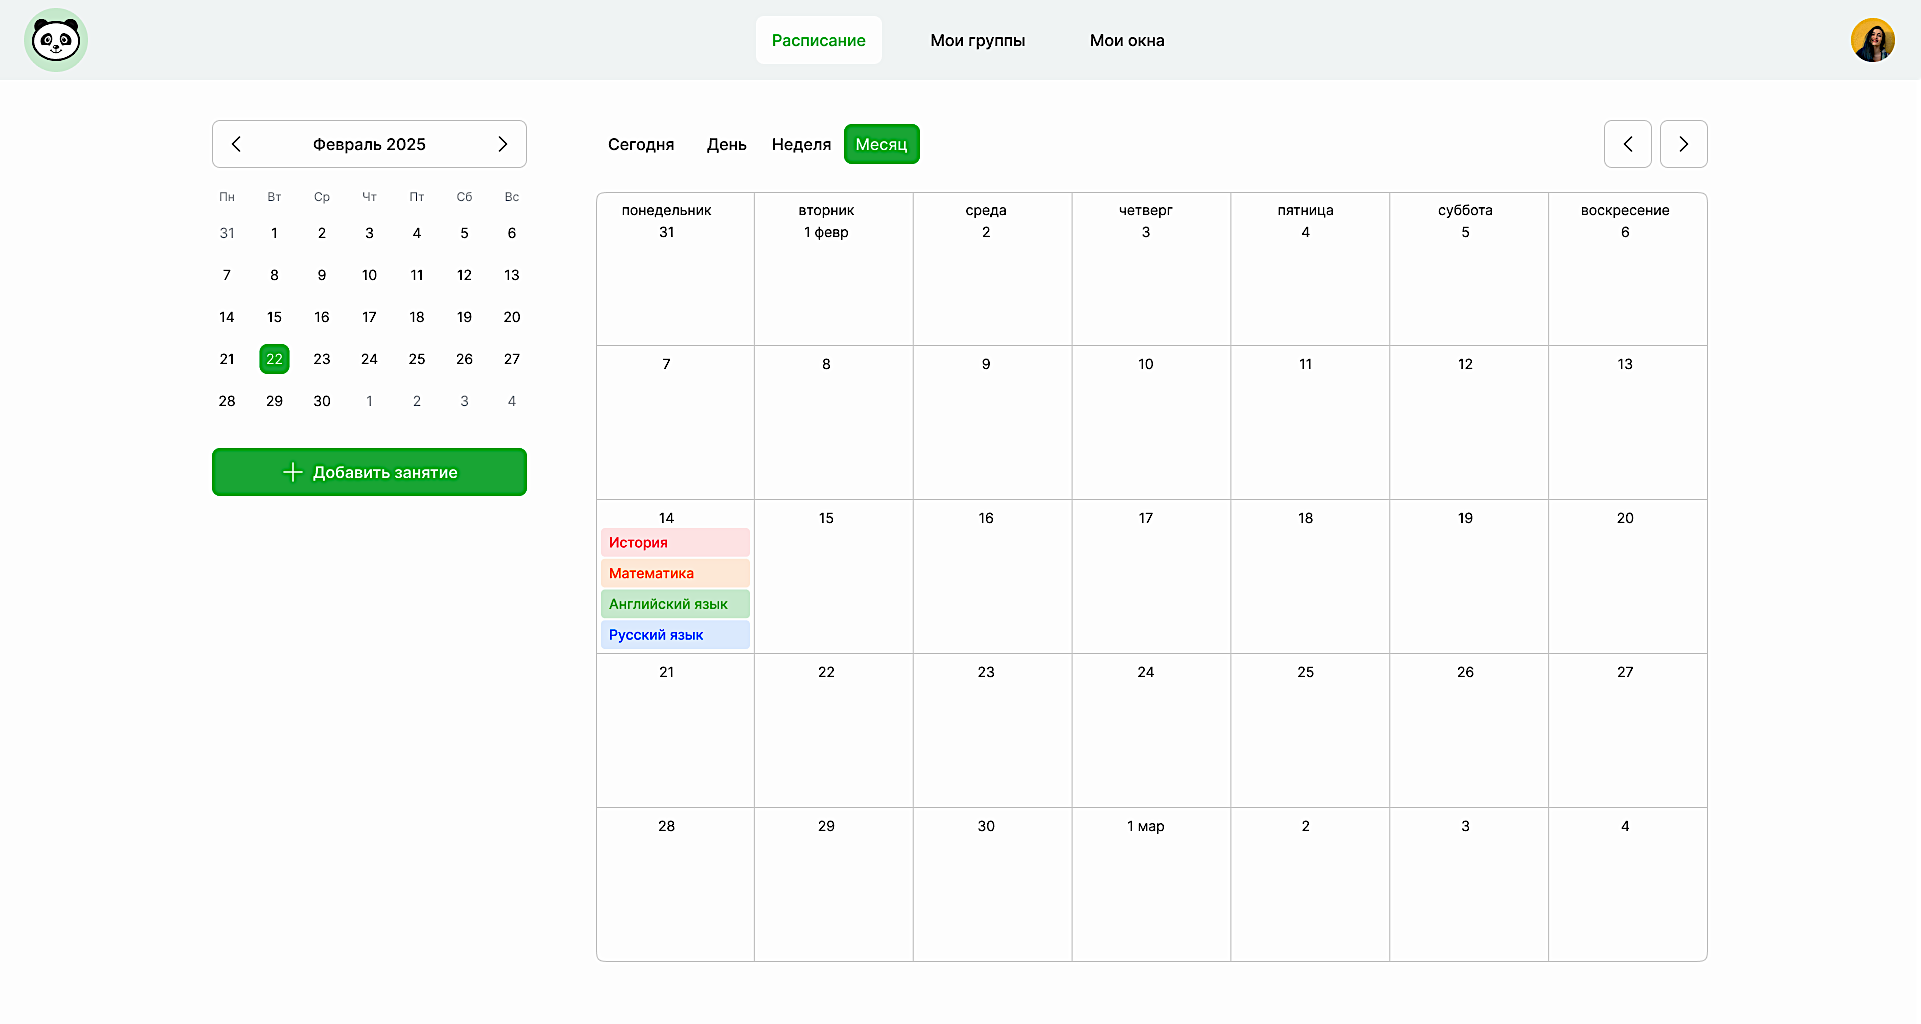
\includegraphics[width=0.7\linewidth]{images/design/Расписание_Месяц.png}}
    \captionof{figure}{Прототип страницы "Расписание". Календарь, месяц}
    \label{fig:enter-label}
}


\mysubsubsection { Создание уникальной айдентики сайта ( UI-kit)}

\mysubsubsection {Обзор внешнего вида всех компонентов, форм и таблиц}

\mysubsubsection {Прототипирование}


\mysubsection {Разработка веб-части}
\mysubsubsection {Поиск оптимального стека технологий необходимый для выполнения требований}

Сегодня для реализации современного, продвинутого и респонсивного фронт-енда недостаточно использование чистого JavaScript, необходимо использование фрейм-ворка.

Согласно [источник], сеодня самыми популярными фреймворками являются:
\begin{itemize}
    \item React
        \begin{itemize}
            \item[+] Наибольшее сообщество и количество готовых решений
            \item[+] Виртуальный DOM для оптимизации рендеринга
            \item[+] Гибкость архитектуры (можно собирать стэк под себя)
            \item[-] JSX может усложнять понимание для новичков
            \item[-] Требует дополнительных библиотек для полноценного стэка (роутинг, state-менеджмент)
            \item[-] Частые изменения best practices
        \end{itemize}

    \item Angular
        \begin{itemize}
            \item[+] Полноценный MVC-фреймворк "из коробки"
            \item[+] TypeScript поддержка на уровне ядра
            \item[+] Хорошая структура для больших enterprise-проектов
            \item[-] Сложная кривая обучения
            \item[-] Громоздкая архитектура для небольших проектов
            \item[-] Менее гибкий по сравнению с React/Vue
        \end{itemize}

    \item Svelte
        \begin{itemize}
            \item[+] Нет виртуального DOM (компиляция в нативный JS)
            \item[+] Простейший синтаксис и минимальный boilerplate
            \item[+] Отличная производительность
            \item[-] Меньшее сообщество и экосистема
            \item[-] Менее подходит для сложных state-зависимых приложений
            \item[-] Проблемы с масштабированием в больших проектах
        \end{itemize}

    \item Vue
        \begin{itemize}
            \item[+] Плавная кривая обучения
            \item[+] Гибкость: можно использовать как целиком фреймворк, так и частично
            \item[+] Оптимальная производительность (комбинация Virtual DOM и реактивности)
            \item[+] Отличная документация
            \item[-] Меньше корпоративных решений
        \end{itemize}
\end{itemize}

Я выбрал Vue.js из-за следующих преимуществ для учебного проекта:

\begin{itemize}
    \item Простота интеграции:
    \begin{itemize}
        \item Легко добавить в существующий проект
        \item Возможность постепенного внедрения
    \end{itemize}
    
    \item Композиционный API:
    \begin{itemize}
        \item Лучшая организация кода по сравнению с Options API
        \item Проще выносить логику в reusable-функции
    \end{itemize}
    
    \item Оптимальная производительность:
    \begin{itemize}
        \item Новая реактивная система на Proxy
        \item Tree-shaking из коробки
    \end{itemize}
    
    \item Экосистема:
    \begin{itemize}
        \item Vue Router для навигации
        \item Pinia/Vuex для state-менеджмента
        \item Vue-CLI-Service для мгновенного hot-reload
    \end{itemize}
    
\end{itemize}

\mysubsubsection {Архитектура приложения}

Архитектура клиентской части приложение сформирована с помощью наслоения одних компонентов над другими. С этой схемой можно ознакомиться на рисунке \_.

{
    \centering
    \fbox{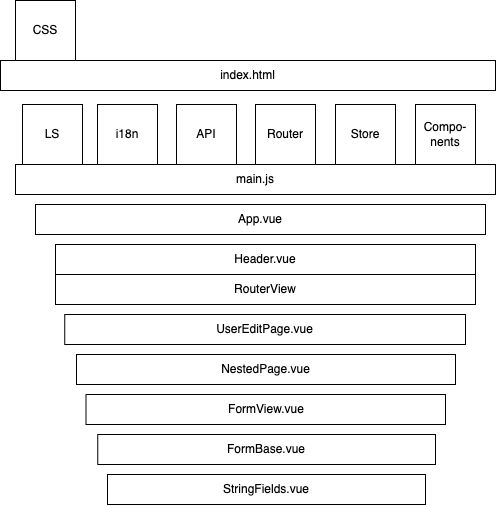
\includegraphics[width=0.7\linewidth]{images/FrontEndLayers.png}}
    \captionof{figure}{Построение компонентов на основе страницы личного кабинета }
    \label{fig:enter-label}
}

Здесь точкой входа является файл index.html - к которому монтируется Vue js приложение, а также все CSS стили.

Монтирование самого приложения происходит в файле main.js. В нем регистрируютяс все используемые глобальные модули для работоспособности приложения:

\begin{itemize}
    \item LS (LocalStorage)

    Локальное хранилище данных в браузере. Обеспечивает хранение данных до тех пор, пока пользователь не очистит кеши страницы или не зайдет под инкогнито.
    \item i18n

    Модуль позволяет реактивно изменять локаль приолжения, переключаясь моментально между языками в интерфейсе.
    \item API

    По своей сути является объектом, который разделяет API для использования внутри фронта на смысловые части. Значениями же являются функции, которые посылают запросы к бекенду.

    \item Router

    Зарегистрированный роутер, позволяющий монтировать определенные View компоненты к URI путям. Также отвечает за навигацию внутри приложения.

    \item Store

    Хранилище данных между различными страницами и компонентами. Позволяет хранить глобальные состояния и описания получаемых полей с бекенда. Является слоем данных

    \item Components

    Зарегистрированные компоненты, позволяющие не импортировать каждый файл при использовании компонента, а предоставив глобальный доступ к ним.
\end{itemize}

Все вышеперечисленные модули глобальны и доступны из всех Vue компонентов под main.js

В данном примере рассматривается страница редактирования данных о пользователе, поэтому имеем RouterView - vue компонент, предоставляющий функционал рендера компонента, основанного на текущей локации пользователя внутри приложения. Все существующие страницы внутри проекта описаны на рисунке \_.

{
    \centering
    \fbox{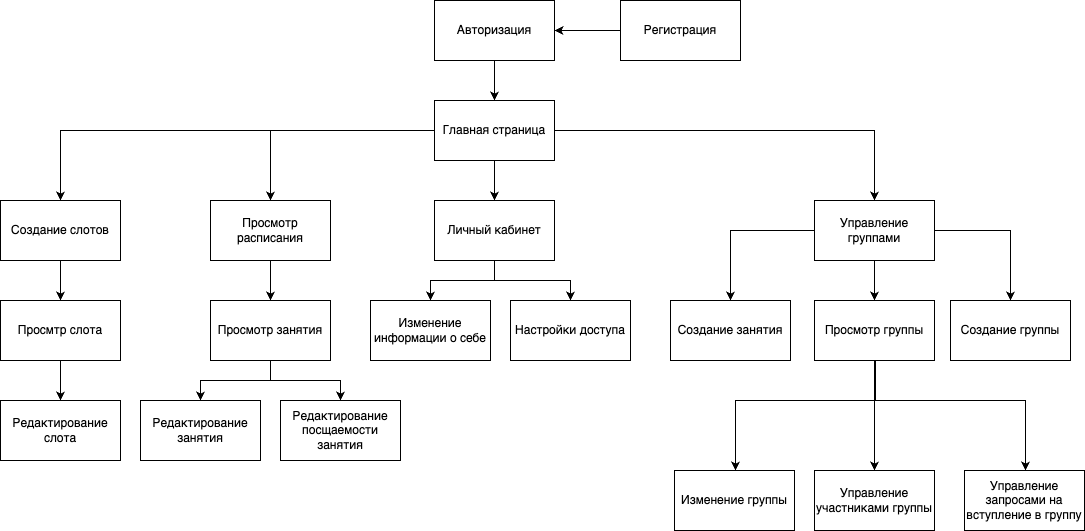
\includegraphics[width=0.7\linewidth]{images/FrotendMap.png}}
    \captionof{figure}{Карта существующих страниц в приложении}
    \label{fig:enter-label}
}


UserEditPage - View компонент, который определяет наполение и функционал этой страницы. В данном примере на странице редактирования мы видим форму FormView.

FormView - общий компонент просмотра, редактирования и создания сущностей. Предоставляет функционал сохранения, отмены и навигации между состояниями формы. C помощью API запрашивает данные о пользователе и отображает их. При изменении данных и нажатии на кнопку сохранить отправляет запрос на обновление данных о пользователе. 

FormBase - основа для FormView. Используя Store, определяет правила для отображения полей внутри формы, а также заполняет их значениями, валидирует их


\mysubsubsection{Архитектура API}

API построено по принципу единой точки входа с последующим роутингом на бэкенде. Основные компоненты:

\begin{itemize}
    \item \texttt{api.help.js} - низкоуровневые HTTP-утилиты
    \item \texttt{api/index.js} - фасад для работы с API
    \item \texttt{Глобальный объект \texttt{api}} - доступен через \texttt{app.config.globalProperties}
\end{itemize}

Транспортный уровень.

Обработка запросов через \texttt{XMLHttpRequest} с дополнительной логикой:

\begin{lstlisting}[language=JavaScript, caption=Обработка запросов,breaklines=true, numbers=left]
const callXhr = ({ url, method, headers, body, ...params }) => 
  new Promise(resolve => {
    const Xhr = new XMLHttpRequest()
    // request config
    Xhr.open(method, url)
    // handlers
    Xhr.send(body)
  })
\end{lstlisting}

Особенности:
\begin{itemize}
    \item Буферизация ответов для контроля размера данных
    \item Единая точка обработки ошибок
    \item Поддержка прогресса загрузки
\end{itemize}

Используется цепочка обработчиков:

\begin{lstlisting}[language=JavaScript, caption=Цепочка обработки,breaklines=true, numbers=left]
const handleRequest = (promise, handlers) =>
  promise.then(res => {
    const handler = handlersByStatusCode[res.statusCode] || defaultHandler
    return handler(res)
  })
\end{lstlisting}

Где \texttt{handlersByStatusCode} содержит специфичные обработчики для каждого HTTP-статуса.


Доступен через Vue-приложение и содержит логически сгруппированные методы:

\begin{lstlisting}[language=JavaScript, caption=Структура API,breaklines=true, numbers=left]
const customApi = {
  auth: {
    login: makeApiFn('/auth/login'),
    register: makeApiFn('/auth/register')
  },
  groups: {
    list: makeApiFn('/groups/list'),
    create: makeApiFn('/groups/create')
  }
  // other modules
}
\end{lstlisting}

Типичный вызов API.
\begin{lstlisting}[language=JavaScript, caption=Пример вызова,breaklines=true, numbers=left]
// In Vue component
this.$api.auth.login(credentials, (response, meta) => {
  if (meta.ok) {
    // ok call back
  } else {
    // errors call back
  }
})
\end{lstlisting}

Особенности реализации:
\begin{itemize}
    \item Автоматическая обработка ошибок: Централизованная система через \texttt{handlersByStatusCode}
    \item Безопасность: Автоматическое добавление JWT-токена из LocalStorage
    \item Гибкость: Поддержка как JSON, так и FormData
    \item Мониторинг: Логирование всех запросов/ответов в консоли
\end{itemize}


API становится реактивным через:

\begin{lstlisting}[language=JavaScript, caption={Интеграция с Vue},breaklines=true, numbers=left]
export const api = new (function() {
  this.install = (app) => {
    app.config.globalProperties.$api = reactive(customApi)
  }
})()
\end{lstlisting}

Это позволяет:
\begin{itemize}
    \item Использовать API в любом компоненте через \texttt{this.\$api}
    \item Получать реактивные обновления при изменении данных
    \item Интегрировать с Vue DevTools
\end{itemize}

Архитектура API обеспечивает единый стиль работы с бэкендом, централизованную обработку ошибок и простую интеграцию с Vue-компонентами при сохранении гибкости для различных сценариев использования.


\mysubsubsection {Механизм авторизации}

Исходя из функциональныз требований, реализовано 3 механизма авторизации: локальный, через Yandex Oauth и Google Oauth.

Внешний вид страницы авторизации представлен на рисунке \_

{
    \centering
    \fbox{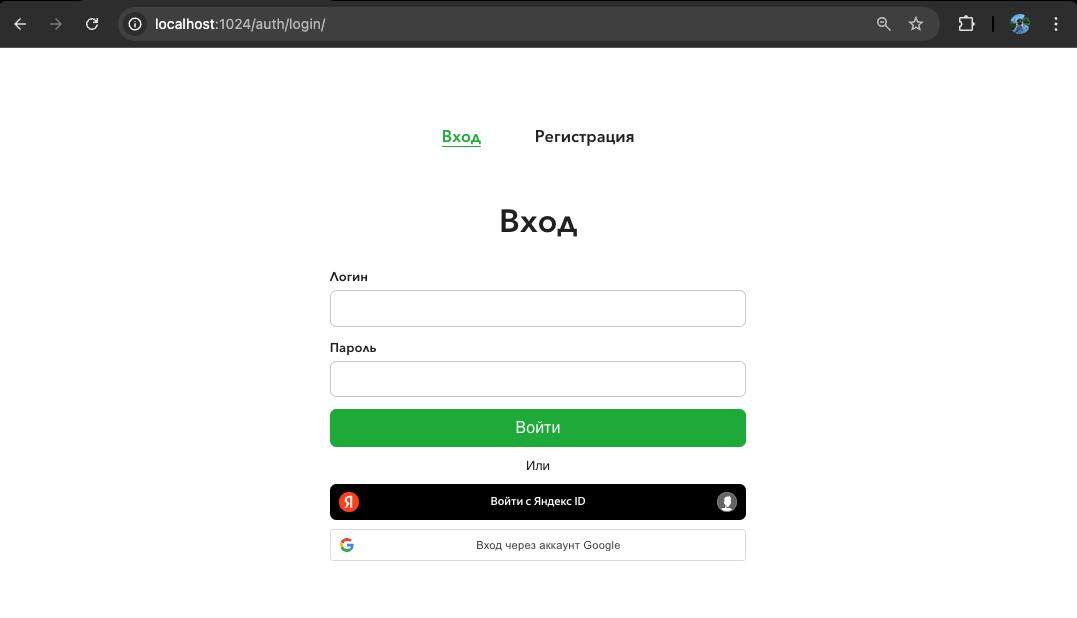
\includegraphics[width=0.7\linewidth]{images/loginPage.jpg}}
    \captionof{figure}{Страница авторизации}
    \label{fig:enter-label}
}

Рассмотрим каждый из них по очереди.

\myparagraph{Локальная авторизация}
\begin{lstlisting}[language=JavaScript, caption=Форма авторизации,breaklines=true, numbers=left]
<FormView displayName="login" action="edit">
    <template #form-bottom="{ entity }">
        <div class="form-bottom-column">
            <BaseBtn @click="authorize(entity)">Войти</BaseBtn>
            Или
            <div id="auth-bottom"></div>
            <div id="auth-bottom2"></div>
        </div>
    </template>
</FormView>
\end{lstlisting}
На листинге 7 представлена форма авторизации. Она рендерит всего 2 поля: поле ввода логина и поле ввода пароля с кнопкой авторизации

При нажатии на кнопку "Войти" срабатывает событие @click и вызвается функция authorize с параметром entity, полученный из формы. Реализация функции на листинге 8.

\begin{lstlisting}[language=JavaScript, caption=Форма авторизации,breaklines=true, numbers=left]
authorize(entity) {
    this.$api.auth.login({ ...entity }, res => {
        if (res?.detail) return
        this.$ls.token = res.access_token
        this.$ls.current_user = res.user_id
        this.$store.commit('setUser', res.user_id)
        this.$router.replace('/home')
    })
},
\end{lstlisting}
Здесь вызывается API метод авторизации login, которому в качестве параметров передаются все полученные значения из формы. Вторым параметром передается callBack функция, которая выполнится асинхронно после успешного выполнения запроса. Она получается в качестве параметра res - результат, полученный с бекенда. 

С бекенда приходит следующее: JWT токен доступа в приложение. Без него доступ невозможен. Также получаем уникальный идентификатор пользователя, для последующих запросов на получение информации о нем в других страницах. Эти данные мы кладем в локальное хранилище браузера, а также в наше внутреннее хранилище, чтобы было удобно доставать его при надобности. 

После чего мы перенаправляем пользователя на главную страницу.


\myparagraph{Авторизация через внешний сервис Яндекс}

Для начала необходимо зарегистрировать приложениие внутри системы авторизации яндекса. Сделать можно это на их сайте https://oauth.yandex.ru/client

При регистрации приложения необходимо указать список данных, которые мы хотим получать от авторизуемого пользователя, а также URL страницы на которую Яндекс будет перенаправлять пользователя после успешной авторизации. (рисунок \_)

{
    \centering
    \fbox{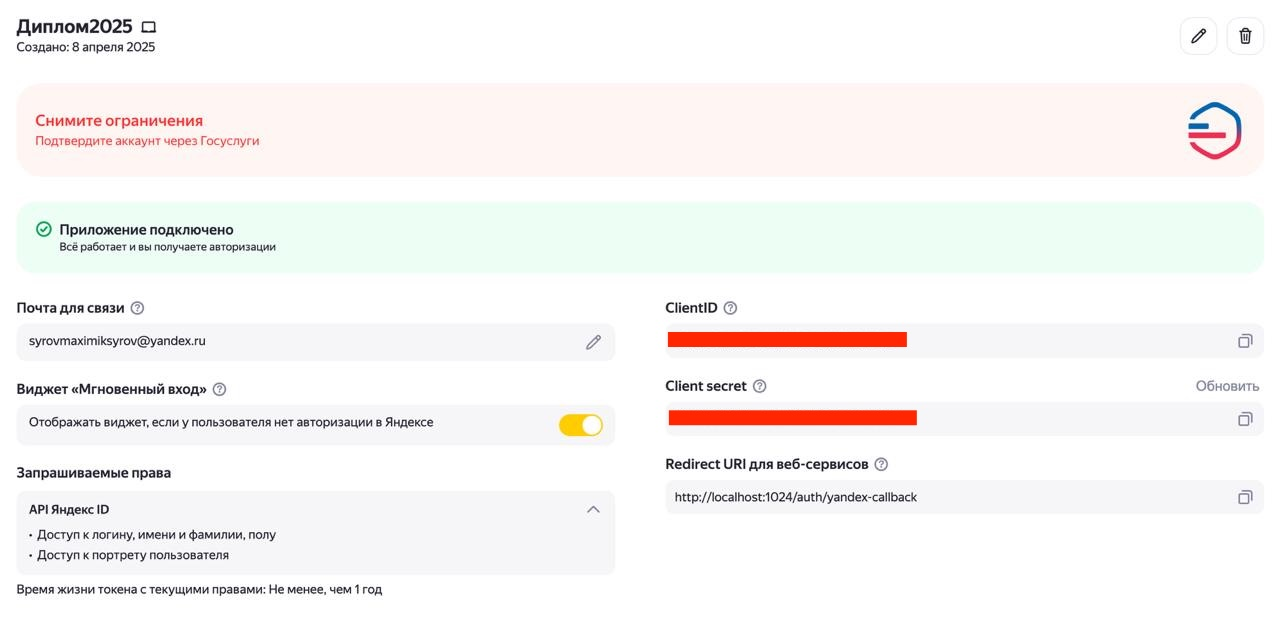
\includegraphics[width=0.7\linewidth]{images/2025-04-09 23.11.44.jpg}}
    \captionof{figure}{Страница с доступом приолжения в Яндекс Oauth}
    \label{fig:enter-label}
}

Теперь необходимо полученный ClientID сохранить в проекте и использовать далее.

Механизм получения данных пользователя через Яндекс:
\begin{enumerate}
    \item Подключить кнопку авторизации в приложение (листинг 9) при создании страницы авторизации Здесь подключается скрипт, предоставленный яндексом, который добавляет в мое DOM дерево свой компонент.
    \item Пользователь нажимает на неё, авторизуясь через свой аккаунт.
    \item С моей страницы на сервер яндекс отправляется запрос на получение токена доступа с помощью моего ClientID (листинг 9, строки 7-13)
    \item После успешной авторизации пользователя, Яндекс перенаправляет пользователя на страницу, указанную в Личном кабинете авторизации и в запросе на получение токена (они обязательно должны совпадать) (листинг 9, строка 12)
    \item Поскольку Яндекс открывает всплывающее окно, а не перенаправляет уже на открытую вкладку, получить токен на той же странице нельзя. Поэтому указана страница auth/yandex-callback, которая, получив токен доступа (листинг 10, строки 2 - 5), запрашивает у яндекса информацию о пользователе и сохраняет её в LocalStorage( листинг 10, строки 7, 8). После чего закрывает всплывающее окно (листинг 10, строка 9)
    \item На старой странице авторизации идет подписка на изменения в LocalStorage под ключом yandex\_user\_data (листинг 11). Таким образом, при изменении значения под этим ключом срабатывает функция, которая получает из LocalStorage данные, расшифровывает их и выполняет последовательно процесс регистрации, а затем авторизации. В случае если пользователь уже зарегистрирован через этот аккаунт, пользователь авторизуется автоматически.
\end{enumerate}
\begin{lstlisting}[language=JavaScript, caption=Процесс инициализации авторизации YandexOauth,breaklines=true, numbers=left]
async initYandexAuth() {
    /* eslint-disable no-undef */
    await this.loadBtnScript(
        'https://yastatic.net/s3/passport-sdk/autofill/v1/sdk-suggest-with-polyfills-latest.js'
    )
    try {
        const { handler } = await YaAuthSuggest.init(
            /* eslint-enable no-undef */
            {
                client_id: YANDEX_CLIENT_ID,
                response_type: 'token',
                redirect_uri: 'http://localhost:1024/auth/yandex-callback',
                display: 'page',
            },
            null,
            {
                display: 'page',
                view: 'button',
                parentId: 'auth-bottom',
                buttonView: 'main',
                buttonTheme: 'light',
                buttonSize: 'm',
                buttonBorderRadius: 8,
            }
        )
        await handler()
    } catch (error) {
        console.error('Yandex auth error:', error)
    }
},
created() {
// other code
this.initYandexAuth()
// other code
}
\end{lstlisting}
\begin{lstlisting}[language=JavaScript, caption=Получение данных о пользователе из Яндекса,breaklines=true, numbers=left]
mounted() {
    const url = new URL(window.location.href)
    const hash = url.hash.substring(1)
    const params = new URLSearchParams(hash)
    const accessToken = params.get('access_token')
    if (!accessToken) return
    this.$api.auth.yandexGetData(accessToken, 'json', data => {
        this.$ls.setItemEncrypt('yandex_user_data', JSON.stringify(data))
        window.close()
    })
},
\end{lstlisting}
\begin{lstlisting}[language=JavaScript, caption=Регистрация и авторизация с данными, полученные из Яндекса,breaklines=true, numbers=left]
this.$ls.subscribe('yandex_user_data', () => {
    const userData = JSON.parse(this.$ls.getItemDecrypt('yandex_user_data'))
    this.$api.auth.register(
        {
            name: userData.first_name,
            // other data
        },
        () => {
            this.authorize({
                login: userData.login,
                password: password,
            })
        }
    )
})
\end{lstlisting}

\myparagraph{Авторизация через внешний сервис Google}

По аналогии с сервисом Яндекса, в Google Oauth необходимо зарегистрировать приложение в их сервисе для управлениями авторизаций https://console.cloud.google.com/ (рисунок \_)

{
    \centering
    \fbox{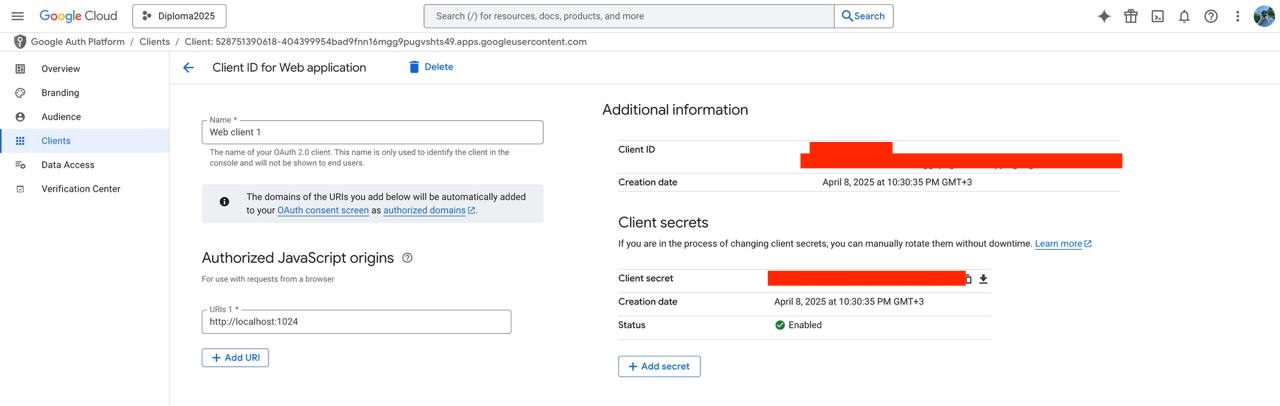
\includegraphics[width=0.7\linewidth]{images/2025-04-09 23.33.10.jpg}}
    \captionof{figure}{Страница с доступом приолжения в Google Oauth}
    \label{fig:enter-label}
}

Процесс авторизации пользователя через Google Oauth схож с методом Яндекса, но несколько проще.

Механизм получения данных пользователя через Google:
\begin{enumerate}
        \item Подключить кнопку авторизации в приложение (листинг 11) при создании страницы авторизации. Здесь подключается скрипт, предоставленный google, который добавляет в мое DOM дерево свой компонент (листинг 11, строка 2)
    \item Пользователь нажимает на неё, авторизуясь через свой аккаунт.
    \item После авторизации пользователем в сплывающем окне, отправляется запрос к серверам Google в котором указывается (листинг 12, строки 6-24):
    \begin{itemize}
        \item client\_id - полученный ClientID при регистрации приложения,
        \item response\_type - то, что мы ожидаем в результате запроса - token, те токен авторизации пользователя. 
        \item scope - это политики доступа, перечисленные через пробел - те данные с которыми авторизуемый пользователь сможет поделиться для приложения.
        \item callback - функция которая отработает в случае успешного запроса к Google.
    \end{itemize}
    \item В случае успешного выполнения запроса, выполняется callback функция. В ней, одним из параметром является зашифрованный с помощью JWT - токен в credentials (листинг 12, строки 7, 8), расшифровав который, можно получить данные пользователя.
    \item С помощью полученный данных пользователя мы также его регистрируем и авторизуем с помозью описанных ранее методов (листинг 12, строки 12 - 24).
        
\end{enumerate}
\begin{lstlisting}[language=JavaScript, caption=Процесс авторизации через Google,breaklines=true, numbers=left]
async initGoogleAuth() {
            await this.loadBtnScript('https://accounts.google.com/gsi/client?hl=ru')
            try {
                /* eslint-disable no-undef */
                await google.accounts.id.initialize({
                    client_id: GOOGLE_CLIENT_ID,
                    callback: ({ credential }) => {
                        const userData = jwtDecode(credential)
                        const password = this.transformPassword(
                            `${userData.sub}-${userData.email.ucFirst()}`
                        )
                        this.$api.auth.register(
                            {
                                name: userData.given_name,
                                // other data
                            },
                            () => {
                                this.authorize({
                                    login: userData.email,
                                    password: password,
                                })
                            }
                        )
                    },
                    response_type: 'token',
                    scope: 'https://www.googleapis.com/auth/userinfo.profile https://www.googleapis.com/auth/userinfo.email	openid',
                    ux_mode: 'popup',
                })
                google.accounts.id.renderButton(document.getElementById('auth-bottom2'), {
                    theme: 'outline',
                    size: 'large',
                    locale: 'ru',
                })
                google.accounts.id.prompt() // also display the One Tap dialog
                /* eslint-enable no-undef */
            } catch (error) {
                console.error('Google auth error:', error)
            }
        },

created() {
    // other code
    this.initGoogleAuth()
    // other code
}
\end{lstlisting}





\mysubsubsection {Разработка UI, обхих компонентов и базовой функциональности}

\mysubsubsection {Компонентное и e2e тестирование}

\newpage
\mysection{Глава}
\mysubsection {Ввод системы в эксплуатацию}
\mysubsection {Сбор обратной связи и QA}
\mysubsection {Определения списка результатов по которым можно определить удовлетворенность пользователей}

\end{document}
